
\documentclass{lmcs}

\usepackage[T1]{fontenc}
\usepackage[utf8]{inputenc}
\usepackage{amssymb,mathtools,booktabs}
\usetikzlibrary{arrows.meta,calc,positioning}
\usepackage{xurl}
\microtypesetup{expansion=false}

\urlstyle{tt}
\Urlmuskip=0mu plus 2mu\relax
\DeclareUrlCommand\AgdaPath{\urlstyle{tt}}

\newcommand{\N}{\mathbb{N}}
\newcommand{\Z}{\mathbb{Z}}
\newcommand{\U}{\mathcal{U}}
\newcommand{\B}{\mathcal{B}}
\newcommand{\Lcal}{\mathcal{L}}
\newcommand{\Gcal}{\mathcal{G}}
\newcommand{\RawDecl}{\mathrm{RawDecl}}
\newcommand{\Cand}{\mathrm{Cand}}
\newcommand{\Layer}{\mathrm{Layer}}
\newcommand{\NormSig}{\mathrm{NormSig}}
\newcommand{\ObSig}{\mathrm{ObSig}}
\newcommand{\Ix}{\mathrm{Ix}}
\newcommand{\Real}{\mathrm{Real}}
\newcommand{\SObl}{\mathrm{SObl}}
\newcommand{\Prim}{\mathrm{Prim}}
\newcommand{\Der}{\mathrm{Der}}
\newcommand{\PrimClasses}{\mathrm{PrimClasses}}
\newcommand{\Foot}{\mathrm{Foot}}
\newcommand{\Shape}{\Pi_{\!\infty}}
\newcommand{\Supp}{\mathrm{Supp}}
\newcommand{\hcomp}{\mathrm{hcomp}}
\newcommand{\hfillop}{\mathrm{hfill}}
\newcommand{\compop}{\mathrm{comp}}
\newcommand{\transp}{\mathrm{transp}}
\newcommand{\OpenExt}{\mathrm{OpenExt}}
\newcommand{\res}{\operatorname{res}}
\newcommand{\ext}{\operatorname{ext}}
\newcommand{\Partial}[2]{\mathrm{Partial}_{#1}(#2)}
\newcommand{\Type}{\mathrm{Type}}
\newcommand{\El}{\mathrm{El}}
\newcommand{\Fib}{\mathrm{Fib}}
\newcommand{\Cext}{C_{\mathrm{ext}}}

\title[Toward Coherence Depth Two]{Toward Coherence Depth Two for Cubical Sealed Extensions}

\author[H.\ Lande]{Halvor Lande}
\address{Independent researcher, Oslo, Norway}
\email{halvor.s.lande@gmail.com}

\keywords{cubical type theory, extension calculus, coherence, univalence}
\subjclass[2012]{Theory of computation~$\rightarrow$~Type theory; Mathematics of computing~$\rightarrow$~Algebraic topology}

\begin{document}

\begin{abstract}
Type-theoretic foundations can grow by sealing globally acting structural
layers: modalities, universe formers, promoted interface packages, and similar
operations whose behavior becomes part of the public core.  Such a layer must
explain how it interacts with already exported structure; we call this residue
its public structural trace.  This paper proves a depth-two theorem for a fixed
cubical sealed-extension calculus.  Unary trace is not enough, because
univalence turns equivalences such as the nontrivial swap of the two-point type
into public paths.  Higher structural trace generated by sealing is not
primitive: it is represented by cubical open-box extension data computed from
lower-arity boundaries.  Consequently the exact realized obligation objects
stabilize at binary trace, and normalized minimal public signatures contain no
primitive structural trace field above binary arity.  The mechanized
development checks the theorem-facing fixed-calculus stack, semantic wrapper
interfaces, and the theorem-map/postulate audit; broader transfer to other
cubical foundations remains conditional on the stated interface.
\end{abstract}
\maketitle

\section{Introduction}

A type-theoretic library can grow in two very different ways.  In the first,
a user defines a new transparent object inside an already fixed foundation.  A
new datatype of trees, for example, need not explain how it interacts with every
old construction in the library before it can be used.  Its dependencies are
local, and the surrounding theory can mostly ignore it.

The second kind of growth is less forgiving.  A foundation can be extended by a
new sealed structural layer: a modality, a universe former, a promoted interface
package, or some other globally acting operation whose public behavior becomes
part of the exported core.  Such an extension is not merely another transparent
term.  Once sealed, it advertises a stable public interface.  It must therefore
explain how it acts on the active structure already present: old type formers,
transport operations, eliminators, computation rules, paths, equivalences, and
comparison data.  This explanatory residue is what we call \emph{public trace}.

The question of this paper is:
\begin{quote}
When a cubical type-theoretic foundation is extended by a sealed, globally acting
structural layer, how much public integration trace must remain primitive after
normalization and opacity?
\end{quote}

We keep one small running example in view.  The old interface exports the
two-point type \(2\) and the univalent swap path
\(p_{\mathrm{swap}}=\mathrm{ua}(\mathrm{swap}):2=2\).  A sealed operation
\(X\) supplies an endomap \(F_2:2\to2\).  The constant-left choice is valid
unary data but fails the binary comparison along \(p_{\mathrm{swap}}\); the
identity choice is the positive control.  Later, after such binary boundary data
is present, an additional generated compatibility becomes a structural horn
whose missing face is supplied by the open-box construction.

The answer proved here is a depth-two theorem for one fixed formal calculus.  In
that calculus, unary trace is not enough: univalence supplies genuine binary
naturality obligations.  But trace above binary arity is not primitive: the
higher structural obligations generated by sealing are cubical open-box extension
problems, and cubical composition and filling compute their missing faces and
fillers.  Thus higher exact obligation factors remain visible in the semantics,
but they disappear from minimal opaque public signatures.

A compact summary is:
\begin{quote}
Binary trace is necessary; higher structural trace is computed from
open-box extensions.
\end{quote}

This summary is deliberately about \emph{structural integration trace}, not about
all higher homotopy in a cubical theory.  The theorem does not say that higher
paths vanish, that user-supplied higher payload is forbidden, or that ordinary
library growth obeys a uniform law.  It says that, for the sealed
extension calculus studied below, the additional public trace forced by sealing a
globally acting structural layer stabilizes at binary trace.

\subsection{Payload, trace, and the running example}

The first distinction is between \emph{payload} and \emph{trace}.  The payload is
what the new sealed layer contributes: a new operation, modality, universe rule,
or promoted structural package.  The trace is the public evidence that this
payload interacts correctly with the already exported interface.

Consider a small old interface containing two objects \(A\) and \(B\), together
with a comparison
\[
  p : A \simeq B
\]
or, in a univalent presentation, a path obtained from such an equivalence.  Now
seal a new globally acting operation \(X\).  There are several levels of public
obligation.

First, there is unary trace: the extension must say how \(X\) acts on individual
old generators such as \(A\) and \(B\).  This is objectwise information.  Second,
there is binary trace: the extension must say that the action of \(X\) respects
old comparison data such as \(p\).  This is not reducible to two unrelated unary
actions, because \(p\) is part of the old public interface.  A sealed action that
acts correctly on \(A\) and \(B\) separately may still fail to commute with the
public equivalence between them.

The running lower-bound example specializes this distinction.  Univalence turns
the boolean swap equivalence into a public path, and transport in the endomorphism
family along that path conjugates an endomap by the swap.  The identity endomap
is fixed, while the constant-left endomap is sent to the constant-right endomap.
Thus the unary fragment can accept objectwise data whose binary sealing
obligation is uninhabited.  Binary trace is a real public obligation, not an
accounting artifact.

This is the first half of the depth-two story:
\[
  \text{depth one is insufficient.}
\]
The constant-left branch proves this lower bound.  The identity branch shows
that binary trace is not an impossible demand, and it is the branch to keep in
mind when the later open-box argument computes additional generated
compatibilities from an already supplied binary boundary.  The second half
explains why the story stops at two.

\subsection{Why higher structural obligations are different}

At first sight, sealing seems to create an infinite tower.  If unary action must
respect binary comparison data, should binary comparison data itself not satisfy
ternary compatibility laws?  Should those laws not satisfy quaternary laws, and
so on?  This is the familiar shape of coherence problems.

Cubical foundations change the accounting.  Their primitive operations are built
to solve open-box extension problems.  Given a partial boundary of a cube and a
compatible base, cubical composition and filling supply the missing face and the
interior filler.  In a CCHM-style core~\cite{cubical} this is the role of the
Kan operations, together with transport and the interval structure.  The point
of the present paper is that the higher structural obligations generated by
sealing have exactly this open-box form.

The relevant higher obligation is not an arbitrary closed higher-dimensional
choice.  It is a \emph{marginal extension problem}.  The lower-dimensional faces
come from the already exported unary and binary trace, together with normalized
public signatures of previous sealed layers.  What appears as a ternary or higher
coherence field is therefore represented as an open box: a partial boundary, a
compatibility condition, a missing remote face, and a filler.  In the fixed
calculus, this open-box extension object is contractible and substitution-stable.
Its canonical point is computed using cubical composition and filling.

This is the key semantic mechanism.  Higher structural obligations are not
ignored.  They remain present in the exact realized obligation object.  But they
are no longer primitive public data, because the calculus computes them from the
lower-arity boundary.  Equivalently, an explicit higher structural field in a
surface presentation can be replaced by a cubical term built from the displayed
boundary, and then erased from the minimal public signature.

In the running example, the constant-left branch has already failed before this
stage.  On the swap-respecting branch, the binary comparison is part of the
public boundary; a later generated compatibility asks whether that lower
boundary extends to a marginal box, not for an unrelated primitive field.

Thus the main theorem has two levels.  At the level of exact realized obligation
objects, higher factors are present but contractible.  At the level of normalized
opaque public signatures, higher structural fields are absent from the primitive
trace count.

\subsection{The fixed calculus proved here}

Let \(C_{\mathrm{ext}}\) be the sealed-extension calculus defined in this paper.
It consists of a CCHM-style cubical core with univalence and Kan
composition~\cite{cubical}, globally acting extension declarations, opaque
public signatures, and a raw adequacy bridge connecting surface presentations to
normalized trace objects.  The definitions of \(C_{\mathrm{ext}}\) are part of
the theorem object.

For an admissible candidate \(X\), write \(\mathrm{Real}_k(X)\) for the exact
realized structural obligation object obtained when public trace is allowed up
to arity \(k\).  Write \(\mu\) for the primitive public trace cost of a normalized
opaque signature.  The central result is:
\begin{quote}
\textbf{Main theorem for \(C_{\mathrm{ext}}\).}
For every admissible candidate \(X\) and every \(k\geq 2\), the restriction map
\[
  \res_{2,k}(X):\mathrm{Real}_k(X)\longrightarrow\mathrm{Real}_2(X)
\]
is an equivalence.  Its inverse \(\ext_{2,k}(X)\) is constructed by adjoining,
in dependency order, the canonical total open-extension witnesses for the
higher structural obligations generated above binary arity.
Moreover, every \(\mu\)-minimal normalized public signature contains no primitive
structural trace field of arity greater than two.  Unary trace is insufficient in
general, as witnessed by the two-point swap obstruction.
\end{quote}

The theorem should be read as an exact-depth statement for a fixed calculus:
\[
  \begin{gathered}
  \text{binary trace is necessary,}\\
  \text{and binary trace is sufficient for primitive public structural integration.}
  \end{gathered}
\]

\subsection{Scope and non-goals}
\label{subsec:scope-nongoals}

The theorem is intentionally scoped.  It is a theorem about the fixed calculus
\(C_{\mathrm{ext}}\), not a claim that this is the only possible formalization
of sealed cubical extension, nor that every Cubical Agda program~\cite{cubical-agda}
automatically interprets into it.  The result also does not say that all higher
filler spaces in Homotopy Type Theory are contractible.  The contractible
objects are the theorem-facing structural open-box extension fibers generated by
this calculus.  User-supplied higher payload, raw higher homotopy, and
non-structural mathematical data remain outside the primitive-trace accounting
unless they are exported as sealing-generated structural integration fields.

The sufficiency direction is proved by the structural horn-to-open-box theorem,
the open-box contractibility theorem, and the computational replacement theorem
for explicit higher structural fields.  The necessity direction is proved by the
univalent boolean-swap obstruction.

The transfer interface isolates the corresponding adequacy criterion: a surface
calculus or cubical foundation inherits the theorem when it admits a faithful
interpretation preserving semantic admissibility, primitive-versus-derived trace
status, historical support, horn-computational replacement, and public trace
cardinality.


\subsection{What the paper proves, and what remains conditional}

The contribution of the paper is a theorem stack for the fixed calculus
\(C_{\mathrm{ext}}\), together with a transfer interface for broader systems.

First, the paper defines a raw sealed-extension calculus that separates payload
from public trace, primitive fields from derived horn-computational fields, exact
realized obligation objects from \(\mu\)-minimal public signatures, and exact
obligation depth from primitive public signature depth.

Second, it proves that every higher structural obligation generated by sealing is
represented as a theorem-facing open-box extension object.  These open-box
extension fibers are contractible and substitution-stable in the fixed cubical
core.  This is the semantic reason that higher exact factors do not contribute
primitive public trace.

Third, it proves a computational replacement theorem.  An explicit higher
structural field in a presentation elaborates to a cubical term, built from
composition, filling, and transport, using only its lower-arity boundary data.
After normalization, the explicit field is absent from the \(\mu\)-minimal public
signature.

Fourth, it proves exact structural integration depth two for \(C_{\mathrm{ext}}\):
\(\mathrm{Real}_k(X) \simeq \mathrm{Real}_2(X)\) for \(k\geq 2\), with no
primitive public trace above binary arity, while the swap obstruction shows that
unary trace alone is insufficient.

Finally, the accompanying Cubical Agda development checks the theorem-facing
fixed model stack: raw normalization and trace accounting, structural horn
decoding, the open-box and horn-computation packages, computational replacement,
wrappers for exact depth, lower-bound witnesses, 2D-foundation wrappers,
semantic wrapper interfaces, and audit fixtures.  The aggregate artifact also
checks the machine-readable theorem map
and reports no local postulates or local primitive declarations in the
theorem-facing import closure.  The development is evidence for the fixed
theorem and for the adequacy program, but the broad transfer claim remains
conditional.  In particular, this paper does not provide a parser or elaborator
theorem for arbitrary Cubical Agda programs, nor a theorem for every cubical
foundation.


\subsection{Related work}
\label{subsec:related-work}

The cubical core used here follows the line of cubical type theory initiated by
Cohen, Coquand, Huber, and M{\"o}rtberg~\cite{cubical}, including the use of
composition, filling, and transport to give computational content to
univalence.  The implementation perspective of Cubical Agda~\cite{cubical-agda}
is a nearby reference point, while the theorem target here is deliberately
smaller than the full surface language.  Cartesian and other cubical
systems~\cite{cartesian-cubical,xtt} provide additional context for how Kan
structure and equality computation may be packaged.

The infinite-tower intuition comes from classical coherence phenomena:
weak higher categories and weak \(\omega\)-groupoids contain coherence data at
all dimensions, and identity types in intensional type theory carry weak
\(\omega\)-groupoid structure~\cite{lumsdaine,vdberg-garner}.  Classical
coherence results for associativity and higher homotopy coherence also shape
that expectation~\cite{maclane-coherence,stasheff-i,stasheff-ii,kraus-vonraumer}.
The present paper is not a strictification theorem for those settings.  Its
claim is narrower: for the generated structural trace of the fixed sealed
extension calculus, higher layers are total open-extension fibers computed from
lower public boundary data.

Two-level type theory and related strict-equality extensions offer a different
way to control coherence: they add a strict equality layer alongside homotopical
equality~\cite{altenkirch-strict,annenkov-2ltt}.  That approach can sidestep
some higher coherence obligations by moving them to the strict layer.  The
collapse here is instead cubical: binary trace remains genuinely necessary in
the univalent layer, while higher sealing-generated structural trace is computed
from lower boundary data.

The opacity and export discipline is indebted to the module-system tradition.
ML-style signatures, functors, sharing constraints, manifest types, and
higher-order modules study how components expose stable interfaces while hiding
implementation details~\cite{macqueen-modules,harper-lillibridge,leroy-manifest,dreyer-higher-modules}.
For proof assistants, module calculi for Pure Type Systems and Coq-style module
implementations make the same modularity issues theorem-facing rather than
purely programming-language-facing~\cite{courant-pts-modules,chrzaszcz-coq-modules,filliatre-letouzey}.
The sealed layers in this paper should be read against that background: the
novel question is not whether abstraction barriers matter, but how much cubical
structural trace such barriers force into the public interface.

Relative to these three lines of work, the contribution is an interface
accounting theorem.  The lower bound uses univalence to show that objectwise
action is not enough; the upper bound uses cubical total-extension
contractibility to show that the higher structural trace generated by sealing is
derived; the module-system analogy explains why only the normalized public
boundary, not private construction history, may be used by later layers.

\subsection{Roadmap}

Section~2 defines the sealed-extension calculus, the payload/trace distinction,
primitive and derived public fields, and the trace-cost invariant \(\mu\).
Section~3 develops normalized public signatures and the raw adequacy bridge,
and Section~4 isolates structural trace roles.  Section~5 proves the open-box
upper bound, replacement theorem, stabilization theorem, and swap lower bound.
Section~6 records the mechanized trusted boundary, and Section~7 concludes.

\section{Fixed sealed-extension calculus}
\label{sec:fixed-calculus}

The preceding section stated the theorem informally: a sealed cubical extension must pay
primitive public trace through binary comparison, but higher structural trace is computed by
cubical horn filling.  This section defines the fixed raw sealed-extension calculus
\(C_{\mathrm{ext}}\), in which payload, trace, opacity, support, and trace cost can be measured
without depending on a particular surface presentation.

\begin{center}
\fbox{\begin{minipage}{0.92\linewidth}
\textbf{Fixed-calculus contract.}
All depth and trace theorems in this paper concern the calculus
\(\Cext\) defined here.  The calculus consists of:
(i) a cubical core with interval, cofibrations, transport, composition,
filling, and univalence;
(ii) raw sealed-extension declarations;
(iii) public-signature extraction and normalization;
(iv) a generated structural-obligation judgment;
(v) depth-indexed obligation signatures \(\ObSig_k\);
(vi) realization objects \(\Real_k\) with restriction maps; and
(vii) a primitive/derived trace classification assigned only after explicit
replacement witnesses have been constructed.  The depth-two theorem is not a
claim about arbitrary Cubical Agda developments or arbitrary cubical
foundations without an adequacy package.
\end{minipage}}
\end{center}

The section has three jobs.  First, it explains what counts as a sealed layer and what is
visible after sealing.  Second, it defines the normalized public signatures on which
primitive trace statements are made.  Third, it records the primitive-class invariants used
to make historical support and trace cost presentation-insensitive.  The depth-two theorem
itself is not proved here: the horn-computing
argument belongs to Sections~4 and~5.  What this section supplies is the accounting language
in which that theorem can be stated.

\subsection{Notation and terminology}

A library state is written \(B\).  Its sealed layers are written \(L_0,L_1,\ldots\), and
\(S(L_i)\) denotes the atomic public signature exported by \(L_i\) after counting
normalization.  A new declaration is written
\[
  e=(\Gamma_{\mathrm{new}},\Gamma_{\mathrm{act}},\Gamma_{\mathrm{cmp}},\sigma).
\]
The component \(\Gamma_{\mathrm{new}}\) contains payload, \(\Gamma_{\mathrm{act}}\) contains
unary action trace, \(\Gamma_{\mathrm{cmp}}\) contains comparison and horn-boundary trace, and
\(\sigma\) selects what is exported through the opaque public interface.

The following vocabulary is used throughout the paper.

\begin{center}
\begin{tabular}{p{0.24\linewidth}p{0.66\linewidth}}
\hline
Term & Meaning in this paper \\
\hline
Sealed extension & A new opaque layer added to the exported foundation or public interface. \\
Payload & The genuinely new mathematical or operational structure supplied by the layer. \\
Trace & Public compatibility data required for the payload to interact with prior exports. \\
Primitive trace & Trace not synthesized by normalization or cubical structural computation. \\
Derived trace & Trace present in a presentation but computed from lower data or generic operations. \\
Counting normal form & The canonical flattened telescope on which public fields are counted. \\
Active basis site & One irreducible primitive class of an earlier normalized public signature. \\
Adequacy boundary & The bridge from richer semantic or surface systems into this raw calculus. \\
\hline
\end{tabular}
\end{center}

Two separations should be kept in mind.  First, payload may be higher-dimensional.  A user
may add higher inductive constructors, path constructors, or other genuinely higher content.
Those are counted as payload when they are part of the new layer's mathematical content.
Only the compatibility data forced by sealing the new layer against old public interfaces is
called structural trace.  Second, exact realized obligation objects and minimal public
signatures are different.  A higher horn obligation may remain present as a contractible exact
factor while contributing no primitive field to the minimal opaque signature.

\subsection{Raw syntax and judgments}

The theorem target is the following raw extension calculus.  Its grammar is deliberately
small:
\[
\begin{array}{rcl}
\multicolumn{3}{c}{i,j,n \in \mathrm{LayerId}}\\
B &::=& \cdot \mid B,L_i,\\
e &::=& (\Gamma_{\mathrm{new}},\Gamma_{\mathrm{act}},
          \Gamma_{\mathrm{cmp}},\sigma),\\
\phi &::=&
  \mathsf{Payload}(q)
  \mid \mathsf{Act}(s)
  \mid \mathsf{Cmp}(s,t,p)
  \mid \mathsf{Horn}_k(\partial),\\
\Sigma &::=& \cdot \mid \Sigma,\phi:T.
\end{array}
\]
Here \(B\) is a monotone state of sealed layers.  The new declaration \(e\) has four parts.
The payload telescope \(\Gamma_{\mathrm{new}}\) introduces the new symbols of the layer.  The
action telescope \(\Gamma_{\mathrm{act}}\) describes unary action on selected old interface
sites.  The comparison telescope \(\Gamma_{\mathrm{cmp}}\) describes binary comparison,
transport, naturality, and horn-boundary data.  The export selection \(\sigma\) records which
elaborated fields are visible after sealing.  The field grammar separates payload from
structural trace: \(\mathsf{Payload}(q)\) belongs to the new mathematical content, while
\(\mathsf{Act}\), \(\mathsf{Cmp}\), and \(\mathsf{Horn}\) are the theorem-facing structural
trace shapes.

The fixed calculus is specified by the following judgments:
\[
\begin{array}{rcll}
  B\;\mathrm{wf} &&& \text{well-formed states},\\
  B\vdash e:\mathrm{RawDecl} &&& \text{raw declarations},\\
  B\vdash e\;\mathrm{adm} &&& \text{admissible declarations},\\
  B\vdash \mathrm{Elab}(e):\mathrm{Cand} &&& \text{elaboration to candidates},\\
  B\vdash \mathrm{Seal}(e):\mathrm{Layer} &&& \text{opaque sealing},\\
  B\vdash N(e):\mathrm{NormSig} &&& \text{normalized public signatures},\\
  B\vdash \phi:\mathrm{RawField} &&& \text{selected public fields before classification},\\
  B\vdash \mathrm{class}(\phi)\in\{\Prim,\Der\}
    &&& \text{post-replacement class},\\
  B\vdash \Supp(\phi)=S &&& \text{historical support}.
\end{array}
\]
An admissible declaration is therefore not just a syntactic tuple.  Its payload, action
clauses, comparison clauses, horn-boundary clauses, and export selection must type-check;
the selected footprint must match the advertised structural action; and the exported interface
must normalize to an opaque public signature.

\begin{figure}[t]
\small
\[
\begin{array}{@{}c@{}}
\dfrac{
  B\;\mathrm{wf}
  \qquad s\in I(B)
  \qquad B,\Gamma_{\mathrm{new}}\vdash a_s:\mathsf{Act}(X,s)
}{
  B\vdash a_s:\mathsf{Unary}(X;s)
}
\;(\textsc{Act})
\\[2.2ex]
\dfrac{
  \begin{gathered}
  B\vdash a_s:\mathsf{Unary}(X;s)
  \qquad
  B\vdash a_t:\mathsf{Unary}(X;t)
  \qquad
  p:s\simeq t\in I(B)\\
  B\vdash b_p:\mathsf{Cmp}(a_s,a_t,p)
  \end{gathered}
}{
  B\vdash b_p:\mathsf{Binary}(X;s,t,p)
}
\;(\textsc{Cmp})
\\[2.2ex]
\dfrac{
  \begin{gathered}
  B\vdash \partial:\mathsf{Boundary}_k(X)
  \qquad k\geq 3\\
  B\vdash h:\OpenExt_k(\partial)
  \end{gathered}
}{
  B\vdash h:\mathsf{Horn}_k(X;\partial)
}
\;(\textsc{Horn})
\\[2.2ex]
\dfrac{
  B\vdash e:\RawDecl
  \qquad
  B\vdash e\;\mathrm{adm}
  \qquad
  B\vdash N(e):\NormSig
}{
  B\vdash \mathrm{Seal}(e):\Layer
  \qquad
  B,\mathrm{Seal}(e)\;\mathrm{wf}
}
\;(\textsc{Seal})
\end{array}
\]
\caption{Core theorem-facing rules of the sealed-extension calculus.  The
judgments use the schematic families \(\mathsf{Act}\), \(\mathsf{Cmp}\), and
\(\mathsf{Boundary}_k\) defined by the raw declaration being elaborated; the
later sections make their normalization and derivedness criteria precise.}
\label{fig:core-rules}
\end{figure}

\begin{defi}[Generated structural obligations]
\label{def:generated-structural-obligations}
For a cubical context \(\Gamma\), a normalized old public signature \(\Sigma\), and a
candidate \(X\), the structural obligations generated by sealing \(X\) over
\(\Sigma\) are the least arity-indexed family of judgments
\[
  \Gamma;\Sigma\vdash \tau\in\SObl_n(X)
\]
closed under the \textsc{Act}, \textsc{Cmp}, and \textsc{Horn} constructors of
Figure~\ref{fig:core-rules}, and stable under weakening, substitution, and
presentation equivalence of \(\Sigma\).  The arity \(n\) is the maximum public
boundary dimension inspected by \(\tau\): action obligations have arity one,
comparison obligations have arity two, and structural horn obligations have
arity \(n\geq 3\).  Payload declarations are not members of \(\SObl_n(X)\)
unless the export selection explicitly reclassifies them as structural
integration trace.
\end{defi}

\begin{defi}[Depth-indexed admissibility]
\label{def:depth-indexed-admissibility}
For \(k\in\mathbb N\cup\{\infty\}\), a candidate \(X\) is
\emph{\(k\)-admissible} when every generated obligation
\(\tau\in\SObl_n(X)\) with \(n\leq k\) has evidence in the corresponding
realized obligation object.  Unary admissibility means \(1\)-admissibility,
binary admissibility means \(2\)-admissibility, and full admissibility means
\(\infty\)-admissibility.  The paper does not define full admissibility by
appealing to the depth-two theorem; the theorem later proves that, for
\(\Cext\), binary admissibility extends canonically to full structural
admissibility.
\end{defi}

\begin{defi}[Raw structural clause classes]
The raw calculus uses three theorem-facing structural clause classes.

A \emph{raw action clause} is a field of \(\Gamma_{\mathrm{act}}\) whose support mentions one
prior opaque interface site and specifies the new payload's unary action on that site.

A \emph{raw comparison clause} is a field of \(\Gamma_{\mathrm{cmp}}\) whose support mentions
two prior interface sites and compares the two induced unary composites.  These include the
transport and naturality squares forced by old public paths or equivalences.

A \emph{raw horn clause} is a field of \(\Gamma_{\mathrm{cmp}}\) whose type presents a higher
structural boundary together with the missing-face and filler package of Section~5.  Raw horn
clauses may occur in exact realized obligation objects.  After the adequacy bridge and the
computational replacement theorem, they are classified as derived trace exactly when their
witness is synthesized by the cubical Kan operations from the lower boundary.
\end{defi}

The last sentence is important.  The word ``derived'' is not meant to be a mere syntactic tag.
The raw syntax records where a horn-shaped structural field appears; Sections~4 and~5 prove
that the relevant fields are computed by explicit cubical operations and therefore disappear
from \(\mu\)-minimal public trace.

\subsection{States, extensions, and public signatures}

\begin{defi}[State]
A \emph{state} or \emph{library} is a monotone context \(B\) closed under derivability.  An
evolution step
\[
  B_n \rightsquigarrow B_{n+1}
\]
adjoins one sealed integration layer, denoted \(L_{n+1}\).
\end{defi}

A state is not the same thing as a source file or an informal collection of lemmas.  It is the
opaque public interface available to future sealed extensions.  Transparent internal
construction may be used to build a layer, but after sealing only the selected normalized
fields of that layer are visible.

\begin{defi}[Surface extensions]
Over a state \(B_n\), a surface extension declaration is a finite quadruple
\[
  e=(\Gamma_{\mathrm{new}},\Gamma_{\mathrm{act}},\Gamma_{\mathrm{cmp}},\sigma),
\]
where \(\Gamma_{\mathrm{new}}\) is a telescope of newly declared payload symbols,
\(\Gamma_{\mathrm{act}}\) is a finite family of unary action clauses against the active
interface, \(\Gamma_{\mathrm{cmp}}\) is a finite family of comparison, transport, or
horn-boundary clauses, and \(\sigma\) specifies which elaborated fields are exported through
the sealed public interface.  The admissible extensions studied in this paper are exactly
those declarations whose intended action is global on a designated finite part of the active
interface.
\end{defi}

\begin{defi}[Elaboration, sealing, and normalized public signature]
Each admissible surface extension declaration \(e\) over \(B_n\) elaborates to a core object
\[
  \mathrm{Elab}(e)
\]
of the fixed cubical core \(C\).  The payload telescope elaborates to new core declarations.
The action and comparison clauses elaborate to fields witnessing interaction with the active
interface.  The opacity component \(\sigma\) selects the public telescope exported after
sealing.

The \emph{normalized public signature} of \(e\) is the counting normal form
\[
  N(e) := N(\mathrm{Elab}(e)).
\]
It is obtained by flattening the exported public telescope, quotienting transparent telescope
isomorphisms, and recording the transparent synthesis candidates generated by definitional
equality, reflexivity, transport along already exported equalities, generic structural
operations of the ambient cubical calculus, and later derived-trace witnesses.  The
primitive/derived split is assigned only after the replacement theorem has supplied those
witnesses.
\end{defi}

\begin{defi}[Presentation equivalence and accounting notation]
\label{def:mu-provisional}
Two admissible surface extensions \(e\) and \(e'\) over the same state are
\emph{presentation-equivalent}, written
\[
  e \approx e',
\]
when their elaborated sealed extensions determine the same public typing judgment up to
definitional equality, canonical telescope isomorphism, and transparent internal
normalization.

Once the replacement theorem has been applied, write
\(N_{\mathrm{tr}}^{\mathrm{prim}}(e)\subseteq N(e)\) for the irreducible primitive trace
schemas in the normalized public signature of \(e\).  The notation
\[
  \mu(e) := \min\{\, |N_{\mathrm{tr}}^{\mathrm{prim}}(e')| \mid e' \approx e \,\}
\]
is reserved here for that later minimal opaque cost.
In the mechanization, the admissible presentation moves are generated by explicit
presentation steps, including reassociation, record splitting and bundling,
currying/uncurrying, transport of fields, transparent alias insertion or deletion, and
duplicate-derived deletion.
\end{defi}

Definition~\ref{def:mu-provisional} is only accounting notation.  The formal
well-definedness of the primitive part used by \(\mu\) is not taken from a raw grammar tag:
it is justified by the computational replacement theorem of Section~3 and by the
\(\mathsf{DerivedTrace}\) witnesses constructed in Sections~4 and~5.  Until those results
have been proved, ``primitive'' and ``derived'' name the two cases of the later canonical
normal form, not extra input data supplied by raw declarations.

The invariant \(\mu\) is deliberately insensitive to packaging.  A trace square does not become
cheaper by being hidden inside a one-constructor record, and it does not become more
expensive by being presented as several equivalent telescope spines.  What \(\mu\) counts is
irreducible primitive public trace after canonical normalization.

\begin{defi}[Candidate]
A \emph{candidate} over a library state \(B\) is a pair
\[
  X=(X_{\mathrm{core}},G_{\mathrm{obl}}),
\]
where \(X_{\mathrm{core}}\) is the mathematical content proposed for addition and
\(G_{\mathrm{obl}}\) is the family of normalized atomic structural obligations induced when
\(X\) is sealed against the active interface of \(B\).  Every admissible surface extension
declaration \(e\) determines such a candidate by elaboration.
\end{defi}

\begin{defi}[Counting normal form and atomic schemas]
\label{def:counting-normal-form}
Every public interface in this paper is counted only up to canonical telescope isomorphism:
reassociation and flattening of iterated dependent sums, splitting or rebundling a
single-constructor record into nested records, and currying or uncurrying iterated function
arguments when these preserve the same sealed typing judgment.  Concretely, an exported
interface is read as a dependent record, equivalently an iterated \(\Sigma\)-type whose field
types may themselves begin with \(\Pi\)-telescopes.  Its \emph{counting normal form} is the
fully flattened telescope obtained by reassociating the \(\Sigma\)-spine and expanding such
record wrappers.

An \emph{atomic schema} is one field of this counting normal form after transparent
telescope isomorphisms have been quotiented.  After the replacement theorem has been
applied, such a field is classified as \emph{derived} when its inhabitant is uniformly
synthesized from earlier fields by definitional equality, reflexivity, transport along
already exported equalities, generic structural operations of the ambient calculus, or a
derived trace witness in the sense of Definition~\ref{def:derived-trace-witness}.  It is
classified as \emph{primitive} when no such transparent synthesis is available in the fixed
calculus.  The cost and basis notions below count primitive atomic schemas after this later
classification; derived schemas may remain present in exact signatures but contribute no
primitive public trace unit.
\end{defi}

\begin{defi}[Core payload size]
For a candidate \(X\), let \(P(X)\) be the finite set of atomic payload schemas appearing in
the counting normal form of the public interface contributed directly by
\(X_{\mathrm{core}}\) before any structural witnesses against earlier layers are added.  Its
cardinality
\[
  \kappa(X) := |P(X)|
\]
is the \emph{core payload size} of \(X\).
\end{defi}

\begin{defi}[Sealed extension]
A \emph{sealed extension} is a candidate whose structural obligations have been discharged
and whose resolved data are exported only through an opaque public interface.  The opacity
invariant is the rule
\[
  \text{future layers may depend on } S(L_i),\text{ but not on the derivation of }\mathrm{Seal}(e_i).
\]
Thus future extensions may use exported payload and trace fields, but they may not inspect
the internal derivations that produced them.
\end{defi}

Opacity is what makes trace visible.  If future layers could freely inspect every proof term and
normalization derivation used to build \(L_i\), then some apparent public trace could be
recovered by peeking behind the interface.  A sealed extension disallows that move: the
normalized public signature is the contract with later layers.

\begin{defi}[Semantic sealed layer and public interface]
At the semantic level the \(n\)th sealed layer may be read as a package
\[
  E_n := (B_n,K_n,T_n,\operatorname{interp}_n).
\]
Here \(B_n\) is the incoming library state, \(K_n\) is the payload telescope contributed by
the new content, \(T_n\) is the resolved structural trace telescope exported after sealing, and
\(\operatorname{interp}_n\) interprets both parts in the ambient cubical foundation.  The public
interface of the sealed layer is the tagged coproduct
\[
  I_n := K_n \sqcup T_n.
\]
For the fixed raw instance, \(K_n\) is the payload part \(S_{\mathrm{core}}(L_n)\) of the
normalized public signature and \(T_n\) is the trace part \(S_{\mathrm{tr}}(L_n)\).  User-supplied
higher constructors and other mathematical content belong to \(K_n\) even when they are
genuinely higher-dimensional; only the integration data induced by sealing the layer against
earlier opaque interfaces belongs to \(T_n\).
\end{defi}

\begin{defi}[Promoted interface package]
A \emph{promoted interface package} over \(B\) is a finite package of constructively
irreducible generators and interaction data that is exported as one new sealed layer.  Such a
package need not modify the reduction rules of the kernel.  What matters is that its public
generators become part of the active exported interface for later sealing steps.
\end{defi}

\begin{defi}[Integration latency]
The \emph{integration latency} of a candidate \(X\) over \(B\) is
\[
  \Delta(X\mid B) := |G_{\mathrm{obl}}|,
\]
the number of irreducible atomic structural obligations that must be resolved before \(X\)
can be exported as a sealed layer.
\end{defi}

\begin{rem}[Refactoring invariance of the counting notions]
Because \(\kappa\), \(\Delta\), and later historical support are computed on counting normal
forms, admissible refactorings such as bundling laws into one record, splitting one interface
into several record shells, exporting curried rather than uncurried arguments, or pushing
transparently derivable witnesses deeper into an internal term do not change the counts.
Only a change in the irreducible primitive fields of the sealed typing judgment changes the
metrics.
\end{rem}

For a sealed layer \(L_k\) obtained from a candidate \(X_k\), we write \(S(L_k)\) for the set
of atomic exported schemas in the counting normal form of its public interface and
\[
  \kappa_k := \kappa(X_k)
\]
for its core payload size.  The indexing is chosen so that \(\Delta_k\) denotes the sealing cost
of \(L_k\).

\paragraph{Transparent user-level code.}
A family \(U\) of transparent definitions, lemmas, or record packages over \(B\) lies outside
the sealed-extension transition when its symbols are definitionally reducible using the
existing operational semantics and are not promoted to a new opaque exported layer.  Such a
development contributes zero integration latency and does not alter the active interface seen
by later sealing steps:
all reductions remain inherited from the pre-existing library, and no new opaque generators are
added to the global interface telescope.  It is ordinary growth inside one state, not a state
transition of the form \(B_n\rightsquigarrow B_{n+1}\).

\begin{defi}[Foundational core extension]
A candidate \(X\) over \(B_n\) is a \emph{foundational core extension} if its payload package is
intended to act globally on the currently active interface: the whole payload telescope
\(P(X)\) is operationally or semantically incomplete until its behavior has been specified
against every basis site in its declared footprint, namely a finite selected set of primitive
classes inside the active exported interface.  Typical examples are extensions of a
universe-decoding apparatus, global modalities presented by explicit modal dependent-type
syntax whose context action must distribute across existing type formers and transports, and
heavily promoted generic interfaces whose exported action is library-wide.
\end{defi}

\begin{rem}
\label{rem:sparse-extensions}
Not every sealed extension is foundational in the sense of the previous definition.  A new
datatype or API layer may be orthogonal to much of the existing library and therefore require
only sparse interaction data.  Such extensions may preserve canonicity without becoming
global operations on earlier layers.  The depth theorem below applies to the structural
obligations generated by the fixed sealing discipline; it is not a universality claim about
all sealed library growth.
\end{rem}

This scope restriction is essential.  Ordinary user-level additions typically enlarge a sparse
DAG of modules, datatypes, or APIs and do not force primitive interaction with unrelated
earlier exports.  Foundational core extensions are the global-operation regime in which the
new sealed layer advertises structural action on a declared part of the active interface.

\subsection{Historical support, primitive classes, and bases}

The trace cost of a new layer depends not on the raw number of old fields but on the number
of old primitive classes that remain visible after normalization.  To make this invariant under
presentation, we choose basis representatives only after quotienting by transparent
derivability.

\begin{defi}[Historical interface]
For \(k\geq 1\), the \emph{historical interface of depth \(k\)} at stage \(n\) is
\[
  I_n^{(k)} := \coprod_{j=0}^{k-1} S(L_{n-j}),
\]
the tagged coproduct of the atomic schemas exported by the most recent \(k\) sealed layers
in counting normal form.
\end{defi}

The tags matter: if two layers happen to export isomorphic-looking fields, they are still
different public sites unless the normalized sealed interface identifies them.

\begin{defi}[Primitive classes and basis families]
\label{def:primitive-bases}
For each sealed layer \(L\), let
\[
  \operatorname{PrimClasses}(S(L))
\]
be the finite set of primitive normal-form classes of the normalized public signature of
\(L\).  Two primitive fields represent the same class exactly when counting normalization
identifies them by transparent generation, definitional equality, uniform polymorphic
instantiation, transport along already exported equalities, or the generic structural
operations quotiented in Definition~\ref{def:counting-normal-form}.

A \emph{basis family} \(S_{\mathrm{bas}}(L)\) is a chosen transversal of
\(\operatorname{PrimClasses}(S(L))\), that is, one representative primitive field from each
primitive normal-form class.  For \(k\geq 1\), once a basis family has been chosen for each of
the layers \(L_n,\ldots,L_{n-k+1}\), the associated \emph{historical basis of depth \(k\)} at
stage \(n\) is
\[
  I_{n,\mathrm{bas}}^{(k)} := \coprod_{j=0}^{k-1} S_{\mathrm{bas}}(L_{n-j}).
\]
Its elements are the basis sites on which a globally acting extension is primitively specified.
\end{defi}

\begin{thm}[Canonical primitive classes determine bases]
\label{thm:canonical-bases}
For every sealed layer \(L\) in counting normal form, basis families in the sense of
Definition~\ref{def:primitive-bases} exist.  If \(S_{\mathrm{bas}}(L)\) and
\(S'_{\mathrm{bas}}(L)\) are two such basis
families, then projection to primitive normal-form classes identifies a canonical bijection
\[
  S_{\mathrm{bas}}(L) \cong S'_{\mathrm{bas}}(L).
\]
Consequently the cardinality \(|S_{\mathrm{bas}}(L)|\) is exactly
\(|\operatorname{PrimClasses}(S(L))|\), depends only on the canonical normalized public
signature of \(L\), and for every depth \(k\) the historical basis cardinality
\(|I_{n,\mathrm{bas}}^{(k)}|\) is independent of the chosen transversals and stable under
presentation-equivalent replacement of the participating layers.

Proof contract: the input is a finite normalized public signature; the
constructed output is a canonical primitive class set and any chosen
transversal.  No horn induction or cubical filling is used; the argument is the
finite quotient/transversal argument for counting normal forms.  Lower-arity
dependencies are irrelevant here because the theorem concerns presentation
invariance of primitive classes.  Artifact status: fully mechanized for the
fixed raw calculus.  Without this theorem, historical support and trace cost
would depend on arbitrary basis choices.
\end{thm}

The proof is by finite transversals of the primitive normal-form quotient.  Each class has a
representative, and two choices are canonically matched by projection to the same primitive
class.  Presentation-equivalent layers have canonically isomorphic normalized signatures by
the normalization theorem of Section~3; this isomorphism preserves witnessed primitive/derived
classifications and transparent-generation classes.  Thus the invariant is the primitive
normal-form class set itself, not an arbitrary minimal generating family.

\paragraph{Primitive basis invariants.}
For every sealed layer \(L\) and every presentation-equivalent replacement \(L'\), the finite
primitive class set, any basis-family cardinality, and the historical support and arity of every
primitive trace field are canonically invariant.  This follows by transporting along the
canonical isomorphism of normalized public signatures: Theorem~\ref{thm:canonical-bases}
identifies basis families with primitive normal-form class sets, and the normalization theorem
of Section~3 preserves primitive/derived classifications, transparent-generation classes, and
opaque layer identifiers.

\section{The adequacy boundary and normalized public signatures}

Section~2 defined the raw sealed-extension calculus and the accounting invariant \(\mu\).
Those definitions are intentionally presentation-insensitive: they count only the normalized
opaque public signature exported by a sealed layer.  This section explains how an extension
declaration reaches that normal form.  It is the place where surface syntax, semantic
admissibility, opacity, and trace accounting meet.

The main point is a boundary rather than a slogan: all semantic readings pass through an
\emph{adequacy bridge}, a package of preservation claims connecting a surface or semantic
extension language to the raw normalized signatures counted in Section~2.

The section has three jobs.  First, it states the adequacy package that a surface language or
external cubical foundation must supply in order to inherit the results of the paper.  Second,
it defines the presentation moves that normalization is allowed to forget.  Finally, it proves
that the resulting normalized public signatures preserve exactly the trace information used
later by the horn-computation and depth theorems.

A useful way to read this section is:
\[
\begin{gathered}
\text{surface declaration}
\leadsto
\text{raw admissible declaration}
\leadsto
\text{sealed public interface}\\
\leadsto
\text{normalized public signature}.
\end{gathered}
\]
The depth theorem begins only after the last arrow.  This is what prevents the later
primitive-trace statements from depending on arbitrary choices of record packaging, telescope
bracketing, or explicit versus implicit derived fields.

\subsection{Semantic obligations and the adequacy package}

A sealed extension is not counted merely by looking at the symbols a programmer writes.  The
same public interface may be presented using a record, an iterated dependent sum, a bundled
operation, an unbundled telescope, or an explicit derived compatibility field.  Conversely,
small changes in surface notation may hide a real new primitive public obligation.  The
adequacy bridge identifies which fields are semantic payload, which fields are primitive
public trace, and which fields are derived before \(\mu\) is computed.

\begin{defi}[Semantic structural obligations]
Let \(E_{n+1}\) be a semantic sealed layer over an already sealed state \(B_n\).  A
\emph{semantic structural obligation} for \(E_{n+1}\) is an interface field required to
interpret the new payload of \(E_{n+1}\) against the opaque public interfaces exported by
previous layers.

Unary obligations specify the action of the new payload on one old public site.  Binary
obligations specify compatibility with an old comparison, path, transport, or equivalence
between public sites.  Higher horn-shaped obligations specify the remaining faces of a
higher structural compatibility problem generated by sealing.

User-authored higher payload is not, by itself, structural trace.  If a layer contributes a
higher inductive constructor, a path constructor, or another genuinely higher mathematical
operation, that data belongs to the payload part \(K_{n+1}\).  It becomes structural trace
only when it is a public compatibility field forced by sealing the new layer against old
opaque interfaces.
\end{defi}

The last sentence is one of the most important discipline rules of the paper.  The theorem
is not claiming that higher-dimensional mathematical content disappears.  It is claiming that
higher \emph{structural integration obligations} generated by sealing are represented as
cubical horn-extension problems and therefore do not survive as primitive public trace.

\begin{rem}[Adequacy package and status]
For a general cubical foundation \(\mathcal F\), or for a richer surface language intended to
compile into \(C_{\mathrm{ext}}\), the semantic reading of the theorems is parametric in an
adequacy package \(\mathcal A\).  The package contains the following preservation clauses.

\begin{enumerate}
\item \textbf{Raw soundness.}  Every well-typed surface payload, action, comparison,
transport, or horn-boundary declaration elaborates to the corresponding raw clause class of
\(C_{\mathrm{ext}}\).

\item \textbf{Raw completeness for the fixed sealing discipline.}  Every admissible semantic
structural obligation generated by the chosen sealing discipline is represented by one of the
raw clause classes of Section~2: payload, unary action, binary comparison, or structural horn
boundary.

\item \textbf{Opacity preservation.}  The surface notion of sealing agrees with the raw opaque
export.  After sealing, later layers may use the normalized public interface, but not hidden
transparent derivations except through explicitly exported fields or through the transparent
operations admitted by counting normalization.

\item \textbf{Support preservation.}  Normalization preserves the historical support of every
primitive trace field.  Repackaging may change notation, but it may not turn a field depending
on layers \(i,j\) into one depending on a different public history.

\item \textbf{Primitive/derived preservation.}  Presentation equivalence and normalization
preserve the witnessed primitive/derived classification.  A field is classified as derived
only when the fixed derivability relation supplies a uniform construction from previously
exported lower data.

\item \textbf{Cardinality preservation.}  Payload size, primitive trace size, exported
interface cardinality, and minimal opaque cost \(\mu\) are preserved by the raw-to-normalized
signature bridge.

\item \textbf{Horn-computation preservation.}  Higher structural obligations that the surface
language treats as derived must elaborate to the structural horn-extension packages of
Sections~4 and~5.  In particular, their derived status must be witnessed by the cubical
operations used in the computational replacement theorem, not merely asserted by a tag.

\end{enumerate}

In this paper these clauses are proved or checked for the fixed raw extension calculus.  For
any other system, this list is the transfer target.
\end{rem}

This formulation deliberately makes the broad transfer conjecture smaller and sharper.  The
paper proves a theorem inside \(C_{\mathrm{ext}}\); the adequacy package records exactly what
another system would have to preserve in order to inherit that theorem.


\subsection{Presentation steps and canonical normal forms}

The normalized public signature should not depend on how a programmer packages a public
interface.  A one-constructor record, a flattened telescope, and an equivalent iterated
\(\Sigma\)-type should present the same sealed public data.  Similarly, a derived alias should
not become primitive merely because it was written explicitly.  Presentation equivalence is
therefore generated by a small list of local moves.

\begin{defi}[Presentation-step generators]
Presentation equivalence for admissible declarations is generated by the following local
moves on normalized public telescopes:
\[
\begin{array}{ll}
\mathsf{reassocSigma} & \text{reassociate or flatten an iterated dependent sum;}\\
\mathsf{splitRecord} & \text{split a single-constructor record or shell into fields;}\\
\mathsf{bundleRecord} & \text{rebundle such a field telescope into a record or shell;}\\
\mathsf{curryPi} & \text{turn a product argument into an iterated function telescope;}\\
\mathsf{uncurryPi} & \text{perform the inverse uncurrying step;}\\
\mathsf{transportField} & \text{move a field along an already exported equality;}\\
\mathsf{transparentAliasInsert} & \text{insert a transparently definable alias field;}\\
\mathsf{transparentAliasDelete} & \text{delete such an alias field;}\\
\mathsf{duplicateDerivedDelete} & \text{delete a duplicate derived trace field.}
\end{array}
\]
Their reflexive, symmetric, and transitive closure is the relation
\[
  e \approx e'.
\]
The list is also the scope of the raw bridge.  It covers the raw constructors of
Section~2: payload telescopes, action clauses, comparison and transport clauses, algebraic
payload packages, export selections, and packaged horn-boundary clauses.  It does not include
arbitrary source-language rewrites or parser-level equivalence for Cubical Agda programs.
\end{defi}

The point of this definition is conservative.  Presentation equivalence forgets bureaucracy,
not semantic obligations.  A field may be removed only when it is an alias, a duplicate
derived field, or a different presentation of the same public typing judgment.

\begin{prop}[Counting normalization is stable under presentation steps]
Each generator of presentation equivalence preserves the canonical counting normal form up to
telescope isomorphism, preserves primitive-versus-derived tags, and preserves historical
support.  Consequently, if \(e\approx e'\), then
\[
  N(e) \cong N(e'),
  \qquad
  \operatorname{Prim}(N_{\mathrm{tr}}(e)) \cong
  \operatorname{Prim}(N_{\mathrm{tr}}(e')),
  \qquad
  \mu(e)=\mu(e').
\]

Proof contract: the input is one presentation-equivalence generator; the
constructed output is the canonical isomorphism of normalized public
telescopes, with primitive status and support preserved.  The proof is by case
analysis on the listed generators, not horn induction.  Cubical structure
appears only in the transparent transport and alias moves that counting
normalization already admits.  Artifact status: fully mechanized for the fixed
raw calculus.  Without this proposition, \(\mu\) would be presentation-sensitive.
\end{prop}

Reassociation, record splitting, rebundling, currying, and uncurrying change only the shape of
the public telescope.  After flattening the \(\Sigma\)-spine and normalizing the
\(\Pi\)-telescope, both sides have the same atomic fields up to canonical renaming.

The transport move uses an equality already present in an earlier sealed public signature.
It therefore changes the displayed type of a field but not the irreducible prior public data
on which the field depends.  Transparent alias insertion and deletion add or remove only
fields whose inhabitants are uniformly synthesized from existing exported data.  Such fields
carry derived witnesses and do not contribute to primitive trace cost.  Duplicate-derived
deletion removes a second presentation of a field already classified as derived by such a
witness.

Thus every generator preserves primitive classes and their historical support.  Closure under
reflexivity, symmetry, and transitivity gives the result for \(e\approx e'\).

In the accompanying development this is the theorem-facing contract of
\AgdaPath{Metatheory/PresentationEquivalence.agda},
\AgdaPath{Metatheory/TraceCostNormalForm.agda}, and
\AgdaPath{Metatheory/MuInvariance.agda}.  The paper does not require a global confluence
theorem for arbitrary source syntax.  It requires uniqueness of the counted normal form for
this generated presentation relation, which is exactly the invariant used by the later
primitive-trace results.

\subsection{Elaboration, sealing, and public signatures}

We now connect admissible declarations to the candidate-and-obligation calculus of
Section~2.  The following theorem is the formal version of the pipeline displayed at the
start of the section.

\begin{thm}[Elaboration soundness for sealed exports]
Every admissible surface extension declaration \(e\) over a state \(B_n\) determines:
\begin{enumerate}
\item an elaborated candidate
\[
  X(e) := (X_{\mathrm{core}}(e),G_{\mathrm{obl}}(e));
\]
\item a sealed layer \(L(e)\) exported through the opaque public interface selected by the
export component \(\sigma\);
\item a normalized public signature
\[
  N(e) := N(\mathrm{Elab}(e))
\]
obtained from that exported interface by counting normalization.
\end{enumerate}
In particular, the candidate calculus of Section~2 is the image of admissible surface
extensions under elaboration and sealing.

Proof contract: the input is an admissible surface declaration; the constructed
output is the candidate, sealed layer, and normalized public signature used by
the later obligation calculus.  No structural horn induction is used.  Cubical
operations enter only through the ambient typing and admissibility judgments
that elaborate the declaration.  The output records exactly the public fields
selected by the export component, so later obligations depend on the public
interface rather than on private construction derivations.  Artifact status:
fully mechanized for the fixed raw bridge, and conditional on adequacy for a
broader surface language.  Without this theorem, the syntax counted by the
paper would not be connected to sealed declarations.
\end{thm}

Indeed, the payload telescope \(\Gamma_{\mathrm{new}}\) elaborates to new core declarations,
while \(\Gamma_{\mathrm{act}}\) and \(\Gamma_{\mathrm{cmp}}\) elaborate to the fields witnessing
interaction with the active interface of \(B_n\).  The admissibility judgment says that these
fields type-check and discharge the obligations of the declared structural action; the export
selector \(\sigma\) determines the opaque public telescope; and counting normalization of that
telescope gives \(N(e)\).  These are precisely the candidate and sealed layer used by
Section~2.

\begin{thm}[Adequacy of normalized public signatures]
Let \(e\) be an admissible surface extension over \(B_n\), and let \(L(e)\) be its sealed
export.  Then:
\begin{enumerate}
\item every field of \(N(e)\) comes from a field of the sealed public interface of \(L(e)\);
counting normalization introduces no new primitive public datum;
\item every field of \(N(e)\) is either a payload schema contributed by
\(\Gamma_{\mathrm{new}}\) or a trace schema arising from a resolved structural obligation of
\(X(e)\);
\item every irreducible payload or trace schema visible after sealing occurs as a field of
\(N(e)\);
\item the quantities
\[
  P(X(e)),\quad S(L(e)),\quad \Delta(X(e)\mid B_n),\quad \mu(e),\quad
  \operatorname{ObSig}_k(X(e)),\quad \operatorname{Ix}_k(X(e)),\quad
  \operatorname{Real}_k(X(e))
\]
are exactly the corresponding payload family, public signature, abstract latency, minimal
opaque cost, obligation signature, primitive index set, and realized obligation object computed
from \(N(e)\) and its trace part.
\end{enumerate}

Proof contract: the input is the sealed export of an admissible declaration; the
constructed output is the payload/trace decomposition and the associated
counting and realization objects.  No horn induction is used at this stage.
Cubical operations enter only as transparent operations already admitted by
counting normalization.  The theorem preserves the lower public trace needed by
later horn construction and does not expose private proof terms.  Artifact
status: fully mechanized for the fixed raw calculus and conditional on adequacy
for broader transfer.  Without this theorem, the later depth theorem would have
no justified bridge from normalized public signatures to \(\Real_k\).
\end{thm}

\begin{proof}
The first claim follows from the definition of sealing and counting normalization: the
normalization procedure flattens the exported telescope, quotients presentation artifacts, and
discards uniformly synthesized fields, but it does not invent primitive public data.

The second claim is the surface-language form of the payload/trace decomposition of
Section~2.  After elaboration and sealing, a visible field is either newly introduced
mathematical content of the layer or public evidence that the new content interacts correctly
with earlier opaque interfaces.

For the third claim, observe that counting normalization removes only presentation artifacts
and transparently reconstructible fields.  If an irreducible field is visible after sealing, it is
not uniformly reconstructible from the remaining exported data by the admitted transparent
operations.  It therefore survives into \(N(e)\).

The final claim is bookkeeping.  Section~2 defines payload size, public schema set,
integration latency, minimal opaque cost, obligation signatures, primitive index sets, and
realized obligation objects from normalized public signatures and their induced trace
obligations.  Since \(N(e)\) is the canonical normalized signature of the sealed export, these
abstract quantities agree with the corresponding surface quantities after elaboration.
\end{proof}

The theorem explains why the later sections can stop mentioning surface syntax.  Once a
declaration has crossed the adequacy bridge, all remaining claims are claims about normalized
public signatures and their induced structural obligations.

\paragraph{Irreducible public fields.}
Let \(e\) be an admissible surface extension over \(B_n\), and let \(\phi\) be an irreducible
field of \(N(e)\).  If \(e'\approx e\), then \(N(e')\) contains a canonically corresponding
irreducible field \(\phi'\).  Equivalently, no presentation-equivalent declaration can delete an
irreducible payload or primitive trace schema from the sealed public signature.
This is immediate from the definition of presentation equivalence: it identifies elaborated
sealed extensions only up to definitional equality, canonical telescope isomorphism, and
transparent internal normalization.  If \(\phi\) were absent from \(N(e')\), then \(e'\) would
either omit a public field present in \(e\), contradicting \(e'\approx e\), or reconstruct
\(\phi\) uniformly from the remaining exported data, contradicting irreducibility.

\paragraph{Canonical normalized presentations.}
If \(e\approx e'\), then \(N(e)\) and \(N(e')\) are canonically isomorphic, and their trace
parts are canonically isomorphic.  Consequently every presentation-equivalence class admits a
canonical normalized public signature up to isomorphism, and
\[
  \mu(e)=\left|\operatorname{Prim}(N_{\mathrm{tr}}(e))\right|.
\]
Here presentation equivalence means equality of public typing judgments up to the generated
presentation steps, and counting normal form forgets exactly those differences.  Hence
\(N(e)\) and \(N(e')\) are canonically isomorphic, with corresponding trace subfamilies because
the payload/trace split is part of the sealed public judgment.  The preceding proposition prevents
irreducible primitive trace from being deleted, so the minimum defining \(\mu\) is attained by
the canonical normalized trace signature itself.

\subsection{Computational replacement on canonical trace presentations}

The previous results say that packaging changes do not alter \(\mu\).  The next theorem says
something stronger and more important: an explicitly written higher structural field can
vanish from primitive trace cost when a cubical term reconstructs it from its boundary.
This is the formal expression of the phrase ``derivedness is a theorem, not a tag.''

The theorem below does not itself construct the cubical term.  That construction is supplied
by the horn-to-open-box and open-box computation results of Sections~4 and~5.  What the
theorem proves is that, once the full replacement witness exists in the fixed derivability
relation, the field is not allowed to remain in the \(\mu\)-minimal primitive public
signature.  This is the replacement rule later used by
Definition~\ref{def:derived-trace-witness}.

\begin{thm}[Computational replacement on canonical trace presentations]
Let \(X\) be a candidate over \(B_n\), let \(k\) be a history depth, and let \(S\) be the
canonical normalized trace signature attached to the depth-\(k\) trace family of \(X\).  Let
\(P\) and \(Q\) be two presented trace telescopes whose counting normal forms are \(S\), and
let \(\phi\) be a presented trace field of \(P\).

Suppose \(\phi\) is equipped with a replacement witness of the same shape as
\(\mathsf{DerivedTrace}\): a lower-arity public boundary subfamily \(\partial\phi\), a
cubically synthesized term
\[
  t_\phi(\partial\phi)
\]
built only from \(\mathsf{hcomp}\), \(\mathsf{transp}\), \(\mathsf{hfill}\), definitional
equality, and the transparent structural operations already quotiented by counting
normalization, together with typing and boundary equations, semantic preservation,
allowed-dependency data, substitution stability, and public-normalization compatibility.
Assume this witness shows that after passage to \(S\) the field corresponding to \(\phi\) is
judgmentally reconstructed from lower-arity boundary data.  Then:
\begin{enumerate}
\item \(P\) and \(Q\) are presentation-equivalent representations of the same canonical trace
signature;
\item in the \(\mu\)-minimal part of the canonical normalized trace signature represented by
\(S\), the field corresponding to \(\phi\) is absent as an irreducible primitive trace field;
\item every other irreducible primitive trace field of \(P\) corresponds canonically to one of
\(Q\).
\end{enumerate}

Dependencies: canonical normalized presentations, irreducible-field necessity, the fixed
transparent derivability relation, and public-normalization compatibility of the replacement
witness.

Proof contract: the input is a canonical trace presentation together with a full
replacement witness for one field; the constructed output is the
presentation-equivalent trace presentation in which that field is reconstructed
and no longer primitive.  No horn induction is used here.  Cubical operations
enter only through the supplied witness, whose allowed-dependency component
restricts it to lower-arity public boundary data and transparent structure.
Artifact status: conditional on adequacy, via the normalization and replacement
modules.  Without this theorem, the open-box computation below would give a
semantic center but would not justify lowering the primitive public cost
\(\mu\).
\end{thm}

\begin{proof}
Both \(P\) and \(Q\) normalize to \(S\), so they are two presentations of one canonical public
trace interface.  The hypothesis gives more than a label for \(\phi\): it gives a full
replacement witness.  Its term \(t_\phi(\partial\phi)\) lies in the fixed transparent
derivability relation, reconstructs the normalized image of \(\phi\) from lower-arity
boundary data using only cubical Kan operations and presentation-transparent structural
operations, and carries the typing, boundary, semantic-preservation, dependency, and
substitution evidence needed for the canonical presentation relation.

Consequently the normalized image of \(\phi\) has a transparent derivedness witness rather
than primitive status.  Public-normalization compatibility identifies the presentation with explicit
\(\phi\) and the presentation in which \(t_\phi(\partial\phi)\) is used instead.  The
\(\mu\)-minimal primitive signature retains only irreducible primitive trace fields, so
\(\phi\) is excluded from that primitive part.  Since primitive/derived status and support are
preserved under passage between presentations of \(S\), every other irreducible primitive
field of \(P\) corresponds canonically to one of \(Q\).  Thus computational replacement
changes the presentation of the trace telescope, not the primitive public content measured
by \(\mu\).
\end{proof}

This theorem is the bridge between the cubical argument and the accounting argument.  The
open-box theorem will show that the relevant higher structural fields have terms of the form
\(t_\phi(\partial\phi)\).  The computational replacement theorem then turns that cubical fact
into the public-signature fact that those fields do not contribute primitive trace cost.

\begin{rem}[Mechanized fixed raw bridge]
The formal bridge in the accompanying Agda development is a three-part package for the
fixed raw extension calculus.

\begin{enumerate}
\item Raw admissible declarations are connected, via elaboration and sealing, to canonical
normalized signatures by
\AgdaPath{Metatheory/RawStructuralSyntax.agda},
\AgdaPath{Metatheory/RawStructuralTyping.agda}, and
\AgdaPath{Metatheory/SurfaceNormalizationBridge.agda}.

\item Presentation-equivalent canonical trace normal forms preserve support, primitive cost,
and \(\mu\) by the explicit presentation-step constructors in
\AgdaPath{Metatheory/PresentationEquivalence.agda} and
\AgdaPath{Metatheory/MuInvariance.agda}.

\item The resulting canonical normalized signatures are matched with the counted-interface
quantities by the normalized-signature/counting bridge, and well-typed raw structural clauses
are identified with the horn-generated trace image by
\AgdaPath{Metatheory/SurfaceToHornImage.agda}.
\end{enumerate}

In particular, the computational replacement theorem is formalized at the level of canonical
trace presentations.  The bridge modules connect admissible raw declarations to that
interface and to the counted abstract interface.
\end{rem}

\subsection{The trace-cost dictionary}

For every admissible surface extension declaration \(e\) over \(B_n\),
\[
  \mu(e)
  =
  \left|\operatorname{Prim}(N_{\mathrm{tr}}(e))\right|.
\]
Adequacy of normalized public signatures says that the trace part of \(N(e)\) records exactly
the irreducible public trace schemas arising from resolved obligations of \(X(e)\), while
canonical normalization identifies \(\mu(e)\) with the cardinality of the primitive part of
that trace signature.  The later minimal-signature theorem uses only this identity: once a
higher structural field has a witnessed cubical replacement, it leaves
\(\operatorname{Prim}(N_{\mathrm{tr}}(e))\) and therefore contributes nothing to \(\mu(e)\).

\begin{rem}[Use of the bridge in later sections]
Sections~4 and~5 invoke surface syntax only through the adequacy bridge just described.  Once
an admissible declaration has been identified with its canonical normalized signature and the
corresponding counted-interface data, the later horn and depth theorems are applications of
the abstract candidate-and-obligation calculus.
\end{rem}

\section{Normal forms for structural trace}

The previous section ended at the point where every admissible declaration has been replaced
by a canonical normalized public signature.  We now forget the surface presentation and look
only at the structural trace fields that survive this passage to normal form.  This section is
the bridge between the accounting calculus of Sections~2--3 and the cubical depth theorem of
Section~5.

The bridge has one central purpose.  It explains why the later phrase ``higher trace is
derived'' is not merely a syntactic tag.  A normalized trace field is not classified by its
textual shape alone.  It is classified by the semantic role it plays in the sealed interface,
by the historical support on which its typing derivation genuinely depends, and by whether
there is a uniform construction of the field from already exported lower data.

After normalization, every structural trace field generated by the sealing discipline has one
of three roles:
\[
  \text{unary action trace},
  \qquad
  \text{binary comparison trace},
  \qquad
  \text{higher structural horn package}.
\]
The first two roles may contribute irreducible primitive public trace.  The third role may
remain present in the exact realized obligation object, but in the cubical calculus it is
carried by an explicit horn-computation witness and therefore contributes no primitive field
to a \(\mu\)-minimal public signature.

This is the section-level invariant:
\begin{quote}
Normal form does not erase higher structural obligations; it exposes them as horn packages
whose derivedness must be witnessed.
\end{quote}

\subsection{The three trace roles}

Let \(L_{n+1}\) be a sealed layer over a normalized prior state \(B_n\), and let
\(N_{\mathrm{tr}}(L_{n+1})\) be the trace part of its canonical normalized public signature.
A field of \(N_{\mathrm{tr}}(L_{n+1})\) is structural only when its job is to integrate the new
payload with previously exported opaque interface data.  The same mathematical expression
may have a different status when it is authored as new payload.  For example, a path
constructor contributed by a new higher inductive type is payload; a path witnessing that a
new globally acting operation respects an old exported equivalence is structural trace.

\begin{defi}[Normal structural trace role]
A normalized structural trace field \(t\in N_{\mathrm{tr}}(L_{n+1})\) has one of the following
roles.

\begin{enumerate}
\item \textbf{Unary action trace.}  The field records how the new payload acts on one old
opaque public site.  Its historical support contains one prior public interface component
after counting normalization.

\item \textbf{Binary comparison trace.}  The field records compatibility between two public
routes already determined by unary action, transport, old comparison data, or adjacent
composites through those data.  Its historical support contains two independent public
interface components, or an adjacent binary composite whose two components remain visible in
normal form.

\item \textbf{Higher structural horn package.}  The field records the data of a marginal
higher coherence problem generated by sealing.  Its visible boundary is assembled from
already exported unary and binary trace, together with degenerate faces, reindexings, and
transports that counting normalization treats as transparent.  Its missing face and filler are
represented as an open-box extension package.
\end{enumerate}
\end{defi}

The roles should not be read as a hierarchy of textual arities.  A field whose type begins
with a long telescope may still be unary if that telescope ranges over parameters inside one
old opaque interface.  Conversely, a short-looking comparison may be binary if its typing
derivation uses two independent old public exports.  The invariant is historical support after
all prior layers have been collapsed to their opaque normalized signatures.

\begin{table}[t]
\centering
\small
\setlength{\tabcolsep}{3pt}
\begin{tabular}{p{0.19\linewidth}p{0.25\linewidth}p{0.22\linewidth}p{0.22\linewidth}}
\hline
Normal role & Semantic content & Historical support & Primitive status \\
\hline
Unary action &
Action of the new payload on one exported interface site. &
One prior public field or one primitive class of an old opaque signature. &
Primitive candidate unless transparently generated. \\
\hline
Binary comparison &
Compatibility between two already public routes: actions, transports, equivalences, or
comparison witnesses. &
Two prior public fields, or an adjacent composite trace through them. &
Primitive candidate; necessary in general by the univalent swap obstruction. \\
\hline
Higher horn package &
Boundary, missing face, and filler data for a higher structural obligation generated by
sealing. &
A horn boundary assembled from unary and binary public trace plus transparent structural
faces. &
Derived in the fixed cubical calculus when filled by \(\mathsf{hcomp}\), \(\mathsf{transp}\),
and \(\mathsf{hfill}\). \\
\hline
\end{tabular}
\caption{Normal roles for structural trace fields.}
\end{table}

The table is an accounting table, not a claim that only one-dimensional and two-dimensional
mathematics exists.  Higher-dimensional payload may be primitive payload.  What is at issue
is whether a higher field is forced only to make a sealed structural action coherent with old
opaque public data.  Such fields are the horn packages analyzed below and in Section~5.

\subsection{Unary action trace}

Unary action trace is the most direct form of public integration debt.  A globally acting
sealed layer advertises that its payload can be applied to the active interface already
exported by the foundation.  For each active basis site that lies in the declared footprint,
the normalized public signature must contain either a primitive action field or a transparent
construction of that action from previously exported data.

\begin{defi}[Unary action normal form]
A structural trace field \(a\) is in unary action normal form when there are an old primitive
basis site \(s\in S_{\mathrm{bas}}(L_i)\) and a new payload component \(X\) such that, after
canonical normalization, \(a\) has the form
\[
  a_s : \mathsf{Act}_X(s),
\]
up to the telescope isomorphisms and transparent transports quotiented by counting normal
form.  Its support is \(\mathrm{Supp}(a_s)=\{L_i\}\).
\end{defi}

The notation \(\mathsf{Act}_X(s)\) is schematic.  In a universe example it may be an action
on codes; in a modality example it may be a decoding law; in an algebraic interface it may
be the image of a generator.  What matters is that only one old opaque public site is being
acted on.

Unary action trace is usually primitive because later layers cannot reconstruct objectwise
action on an opaque site unless that action has been exported.  A field of unary shape is
nevertheless not counted as primitive if it is transparently generated.  For instance, an
action on a record projection may be definitionally induced by the action on the record
itself, and an action on a rebundled presentation may be a canonical telescope isomorphism
of an already exported action.  The primitive part of the unary trace consists only of the
irreducible classes left after these transparent identifications.

\begin{lem}[Unary support stability]
If two admissible presentations of a sealed layer are presentation-equivalent, then the unary
action fields of their normalized public trace signatures correspond bijectively up to
primitive-class equivalence.  In particular, presentation equivalence cannot turn an
irreducible unary action on one old opaque basis site into a trace field supported on a
different old layer.
\end{lem}

The normalization moves of Section~3--telescope rebracketing, record--telescope conversion,
definitional expansion and contraction, transparent transport along exported equalities, and
deletion of uniformly synthesized fields--do not change which old opaque primitive class is
being acted on.  Generated or rebundled actions may leave the primitive count, but an
irreducible action on a distinct old basis site cannot move to another site unless the
normalized old interface already identifies them, exactly as recorded by the primitive-class
quotient.

This lemma is one of the reasons the counting invariant \(\mu\) is computed only after
normalization.  Before normalization, a programmer may write several aliases for the same
action or hide an action inside a record field.  After normalization, the unary action role is
read from the old opaque support and is independent of those packaging choices.

\subsection{Binary comparison trace}

Binary comparison trace is the first genuinely cubical obstruction.  It records that two
public routes agree.  The simplest route comparison has the shape
\[
  r_0,r_1 : P
  \qquad\text{and}\qquad
  c : r_0 = r_1,
\]
but the actual endpoints \(r_0\) and \(r_1\) may themselves be composites of action fields,
old transports, decoding equations, univalence paths, or adjacent comparison trace.

\begin{defi}[Binary comparison normal form]
A structural trace field \(c\) is in binary comparison normal form when, after canonical
normalization, it compares two public composites whose irreducible support uses exactly two
old public components.  Schematically,
\[
  c_{s,t} : \mathsf{Cmp}_X(s,t;r_0,r_1),
\]
where \(s\) and \(t\) are old opaque public sites, \(r_0\) and \(r_1\) are the two normalized
routes built from unary action and previously exported trace, and
\(\mathrm{Supp}(c_{s,t})=\{s,t\}\) after quotienting transparent aliases.
\end{defi}

Binary comparison trace is not redundant in univalent cubical settings.  Objectwise action
on the endpoints of an old equivalence does not by itself prove naturality along that
equivalence.  The two-point swap obstruction of Section~5 makes this precise: the old
interface may contain a public path generated by a nontrivial equivalence, and a sealed
operation must say how its action respects that path.  Therefore binary comparison fields
remain primitive candidates in the normal form.

\begin{rem}[Why binary comparison is not merely two unary actions]
A unary field tells us how \(X\) acts on \(s\), and another unary field tells us how \(X\) acts
on \(t\).  A binary field tells us that these actions commute with a public comparison between
\(s\) and \(t\).  In a univalent foundation the comparison may carry real information: an
equivalence can be transported into an equality of types, and the action of \(X\) must be
compatible with that equality.  Thus the binary role records a naturality square, not a pair
of isolated objectwise values.
\end{rem}

Binary fields are nevertheless subject to the same normalization discipline as unary fields.
A comparison obtained by whiskering an already exported comparison with definitional maps
is derived.  A comparison whose two routes become judgmentally equal after normalization is
derived.  A comparison duplicated by a rebundled record field is not counted twice.  But if
the old public interface contains an irreducible comparison and the new sealed action must
respect it, the resulting naturality witness is primitive unless the derivability relation
exhibits a uniform construction.

\begin{lem}[Binary comparison support stability]
Presentation equivalence preserves the primitive-class support of irreducible binary
comparison trace.  It may change the displayed routes by canonical isomorphism or transport,
but it cannot eliminate a genuine binary comparison unless the comparison is transparently
constructed from already exported lower trace.
\end{lem}

The same normal-form argument applies to binary support.  Its two endpoints are route
expressions in the normalized public interface; presentation moves may reassociate, unfold, or
transport them, but after quotienting by transparent operations the pair of independent old
supports remains visible.  If the comparison disappears, the presentation relation has supplied
a transparent construction from previously exported data, so the field is derived and
contributes no primitive trace.  Otherwise it remains an irreducible binary class.

\subsection{Higher trace as a structural horn package}

The third normal role is the one used by the upper-bound proof.  A higher structural field is
not represented as an arbitrary choice of a filler for a completely fixed closed boundary.  It
is represented as a marginal extension problem.  The lower faces are already public.  One
remote comparison face is not yet public.  The obligation is to produce that missing face and
a filler making the resulting open box commute.

This distinction is crucial in a cubical setting.  The space of fillers of a closed higher
boundary need not be contractible.  Cubical types may have genuine higher homotopy.  The
paper therefore does not claim that all higher fillers are unique.  It claims that the
sealing-generated higher structural obligation has open-box extension form, and that the
fixed cubical operations compute the missing structural data needed for public normalization.

\begin{defi}[Structural horn grammar in normal form]
\label{def:structural-horn-grammar}
The higher structural fields generated by sealing are the derivations of a judgment
\[
  \Gamma\vdash H:\mathsf{SHorn}_k(X)
  \qquad (k\geq 3),
\]
where \(\Gamma\) is a normalized public context for the already sealed layers and the
lower-arity trace of \(X\).  Such a derivation carries the following projections:
\[
\begin{array}{rcl}
  \partial(H) &:& \mathrm{Real}_{k-1}(X),\\
  \mathrm{supp}(H) &\subseteq& \{X,L_n,\ldots,L_{n-k+1}\},\\
  \mathrm{miss}(H) &:& \Type,\\
  \mathrm{fill}(H) &:& \mathrm{miss}(H)\to\Type,\\
  \mathrm{export}(H) &:& \{\mathrm{public},\mathrm{transparent}\}.
\end{array}
\]
It also carries a substitution action: for every cubical substitution
\(\sigma:\Delta\to\Gamma\), there is a reindexed derivation
\[
  \Delta\vdash H[\sigma]:\mathsf{SHorn}_k(X[\sigma])
\]
whose projections are the corresponding reindexings of \(\partial(H)\), \(\mathrm{miss}(H)\),
\(\mathrm{fill}(H)\), support, and export status.

The constructors are the following.
\begin{center}
\small
\setlength{\tabcolsep}{3pt}
\begin{tabular}{p{0.19\linewidth}p{0.25\linewidth}p{0.20\linewidth}p{0.24\linewidth}}
\hline
Constructor & Boundary data & Missing face & Filler and public status \\
\hline
Remote comparison
& A boundary \(\partial:\mathrm{Real}_{k-1}(X)\) assembled from public unary trace, public
binary trace, and transparent transports/degeneracies.
& The direct comparison face between \(X\) and the newly exposed remote layer
\(L_{n-k+1}\), compatible with the endpoints of \(\partial\).
& A \(k\)-cell filling the open comparison box; public when the surface presentation exports
it, transparent after replacement. \\
\hline
Degenerate horn
& A lower structural horn with one interval direction degenerated, together with the
degeneracy map.
& The degenerate remote face obtained by applying the degeneracy to the lower missing face.
& The degenerate filler; transparent unless explicitly exported by the surface syntax. \\
\hline
Transported horn
& A structural horn \(H\) and a public path or equivalence used to transport one boundary
face.
& The transported missing face, with endpoint compatibility transported along the same
public path.
& The transported filler; export status inherited from \(H\). \\
\hline
Reindexed horn
& A structural horn \(H\) and a substitution \(\sigma\) of normalized public contexts.
& \(\mathrm{miss}(H)[\sigma]\).
& \(\mathrm{fill}(H)[\sigma]\); export status inherited from \(H\). \\
\hline
\end{tabular}
\end{center}
The element presented by such a derivation is the telescope
\[
  \sum_{\gamma:\mathrm{miss}(H)} \mathrm{fill}(H)(\gamma).
\]
\end{defi}

The remote-comparison constructor is the only constructor that introduces a genuinely new
higher structural obligation.  The degenerate, transported, and reindexed constructors record
the closure conditions needed for substitution stability and presentation invariance.  They do
not introduce new payload and do not make derivedness true by declaration.

\begin{prop}[Structural horn induction]
\label{prop:structural-horn-induction}
To prove a property \(P(H)\) of every sealing-generated structural horn, it is enough to prove
the remote-comparison case and show that \(P\) is preserved by the degenerate, transported,
and reindexed constructors.  If \(P\) includes equations for
\(\partial(H)\), \(\mathrm{miss}(H)\), \(\mathrm{fill}(H)\), support, or export status, the
preservation clauses must use the displayed substitution and transport actions.
\end{prop}

This is the ordinary eliminator for the grammar of
Definition~\ref{def:structural-horn-grammar}, with the projection equations included as
computation rules for the four constructors.

The notation is intentionally close to the later definition of \(H_k(\partial)\).  This
section classifies the normal role; Section~5 proves by the induction principle that the
corresponding cubical open-box extension object is contractible and substitution-stable in
the fixed calculus.

\begin{rem}[The boundary is public]
The boundary \(\partial_h\) is not hidden derivation state.  It is built from the normalized
public signature exported by earlier layers and from the lower-arity trace of the current
sealed layer.  This is why a later layer can reuse the horn computation without reopening the
opaque proof that produced the current layer.  If the boundary of a proposed higher field
depends on private construction details not present in the normalized public interface, then
that field is not a well-formed structural horn package for the present calculus.
\end{rem}

A useful mental picture is the first nontrivial case.  Suppose the new layer has unary action
on a recent public site and binary comparison against an adjacent public comparison.  When a
further remote layer is exposed, the already exported unary and binary data determine all
but one face of a three-dimensional compatibility box.  The remaining face is the direct
remote comparison.  The structural horn package asks for that face together with a filler.
The cubical theorem later says that this package is computed from the displayed boundary by
the ambient Kan operations.

\subsection{Derivedness witnesses}

The word ``derived'' is safe only when accompanied by a witness.  In this paper a higher
structural field is derived because there is a uniform computation that reconstructs it from
its lower boundary.  The witness is part of the normalized role, and the proof of its adequacy
is discharged by the open-box theorem of Section~5.

\begin{defi}[Derived trace witness]
\label{def:derived-trace-witness}
Let \(h\) be a structural horn package with visible boundary \(\partial_h\).  A
\emph{derived trace witness}, written \(\mathsf{DerivedTrace}(h)\), consists of:
\begin{enumerate}
\item lower public boundary data \(\partial_h\) assembled from already exported unary and
binary trace plus transparent structural operations;
\item a replacement cubical term
\[
  t_h(\partial_h)
    : \sum_{\gamma:\Gamma_{\mathrm{miss}}(\partial_h)}
        \mathsf{Fill}_{\partial_h}(\gamma),
\]
constructed uniformly from the visible boundary using the structural operations admitted by
the fixed calculus, in particular composition, transport, and filling;
\item typing and boundary agreement equations showing that the computed missing face and
filler have the presented field's type and restrict to the displayed visible faces;
\item a semantic preservation proof identifying the explicit presentation of \(h\) with the
replacement term in the realized obligation object;
\item an allowed-dependency proof that \(t_h\) uses only lower boundary data and the fixed
transparent cubical operations;
\item substitution stability: for every substitution \(\sigma\), the reindexed computation
\(\sigma^*t_h(\partial_h)\) agrees with the computation on the reindexed boundary
\(t_h(\sigma^*\partial_h)\), up to the canonical equality of the cubical structure;

\item public-normalization compatibility: replacing an explicitly presented field \(h\) by
\(t_h(\partial_h)\) gives a presentation-equivalent normalized public signature in which
\(h\) is not a primitive trace field.
\end{enumerate}
\end{defi}

The term \(t_h\) is the formal content behind the phrase ``computed horn''.  In the fixed
cubical calculus, Section~5 constructs \(t_h\) by turning the structural horn package into an
open-box extension problem and applying the cubical composition and filling operations.  The
transport component aligns the computed face with the already exported comparison data.
The filling component supplies the interior cell.

\begin{rem}[Derived is not a color on syntax]
It would be unsatisfactory to define a raw syntax constructor
\(\mathsf{derivedHorn}\) and then conclude that all higher trace is derived.  The normal-form
judgment used here is stronger.  A higher field may be assigned the horn role only when its
boundary is public and its derivedness obligation is a theorem-facing computation problem.
For the fixed cubical calculus, the computation is discharged by the open-box theorem.  For a
different surface language or foundation, the adequacy package must preserve this witness.
\end{rem}

This is also where the paper's two notions of depth begin to separate.  A horn package may
remain present as an exact obligation factor: the realized object still contains the type of
missing-face-and-filler data.  Once a derived trace witness has been supplied, however,
that package is absent from the primitive part of the normalized public signature.  Thus
higher exact factors can be present and contractible while higher primitive public fields are
eliminated.

\paragraph{Primitive status of the three roles.}
Assume every normalized higher structural horn package in a sealed declaration carries a
derived trace witness.  Then the primitive part of the normalized structural trace
signature is contained in the union of unary action trace and binary comparison trace:
\[
  \operatorname{Prim}\bigl(N_{\mathrm{tr}}(L_{n+1})\bigr)
  \subseteq
  \operatorname{Act}_{\mathrm{prim}}(L_{n+1})
  \sqcup
  \operatorname{Cmp}_{\mathrm{prim}}(L_{n+1}).
\]
Equivalently, no higher structural horn package contributes an irreducible primitive public
trace field to \(\mu\).
By the trichotomy of normal roles, each normalized structural trace field is unary, binary, or
horn-shaped.  Unary and binary fields remain primitive exactly when they are not removed by
transparent generation, canonical telescope isomorphism, or presentation equivalence.  A
horn-shaped field with a derived trace witness is uniformly replaceable by
\(t_h(\partial_h)\), and public-normalization compatibility identifies the presentation with the
explicit field with the one in which the field is synthesized.  Counting normal form therefore
assigns no primitive trace cardinality to that horn field.

The proposition is deliberately conditional.  Section~4 supplies the normal-form
classification and states what a derivedness witness must contain.  Section~5 proves that the
structural horn packages generated by the fixed cubical sealed-extension calculus have such
witnesses.

\subsection{Payload is not reclassified as trace}

The theorem is about public structural integration obligations, not about a collapse of
higher mathematics.  This distinction is easiest to lose precisely at the point where higher
horn packages appear.  The normal-form discipline therefore includes a payload exclusion
rule.

\begin{defi}[Payload exclusion]
A field belongs to payload rather than structural trace when it is authored as new semantic
content of the sealed layer and is not forced merely by the requirement that the new payload
act coherently on the old opaque interface.  In particular, the following are payload when
introduced as part of the new layer:
\begin{enumerate}
\item new operations, type formers, modalities, or universe constructors;
\item algebraic laws internal to the new operation;
\item higher inductive constructors or higher path constructors contributed as new
mathematical structure;
\item user-specified higher cells whose boundary is internal to the new payload rather than
assembled from prior public trace.
\end{enumerate}
Such fields are counted by the payload invariant \(\kappa\), not by the structural trace cost
\(\mu\), unless the sealing discipline separately requires public integration trace for their
action on old interfaces.
\end{defi}

The exclusion rule prevents a misleading reading of the depth-two theorem.  A layer may
export a primitive three-dimensional constructor as payload.  The theorem says only that the
additional structural coherence required to integrate that constructor with the existing
sealed interface is normalized as unary action, binary comparison, and derived horn
computation.  It does not say that the constructor itself is derived or absent.

\paragraph{No payload-to-trace leakage.}
Canonical normalization preserves the distinction between payload fields and structural trace
fields.  A payload field can be accompanied by structural trace explaining its action on old
interfaces, but the payload field itself is not moved into \(N_{\mathrm{tr}}\) merely because it
has higher arity or higher dimension.
The normalized public signature decomposes into payload and trace parts before primitive trace
cost is computed.  Presentation moves may rebundle a payload field, unfold a record containing
it, or transport it along an exported definitional equality, but they do not change its semantic
role as new content of the sealed layer.  A field enters the trace part only when its typing
judgment is an integration obligation against previously exported opaque data; higher-dimensional
payload may increase \(\kappa\), while induced compatibility fields are classified separately.

\subsection{Role uniqueness and presentation invariance}

The normal roles are useful only if they are stable under the presentation moves already
quotiented by the adequacy bridge.  The following proposition records the invariant that is
used implicitly whenever later sections reason about ``the'' action part, comparison part, or
horn part of a normalized trace signature.

\begin{prop}[Trace-role normal form]
Every structural field in the canonical normalized trace signature of an admissible sealed
layer has a unique normal role, up to the primitive-class quotient of Section~2 and the
presentation equivalence of Section~3.  Presentation-equivalent declarations have canonically
isomorphic role decompositions:
\[
  N_{\mathrm{tr}}(e)
  \cong
  N_{\mathrm{tr}}(e')
  \quad\Longrightarrow\quad
  \begin{cases}
    \operatorname{Act}(e) \cong \operatorname{Act}(e'),\\
    \operatorname{Cmp}(e) \cong \operatorname{Cmp}(e'),\\
    \operatorname{Horn}(e) \cong \operatorname{Horn}(e').
  \end{cases}
\]
The isomorphisms preserve historical support and primitive/derived status.

Proof contract: the input is a canonical normalized trace signature; the
constructed output is its unique action/comparison/horn role decomposition.
The proof is case analysis on normalized support and on the structural horn
grammar.  Cubical operations enter only as transparent transports already
quotiented by presentation equivalence.  The lower-boundary condition is the
public support calculation after opacity.  Artifact status: fully mechanized
for the fixed raw calculus.  Without this proposition, the later replacement
theorem would not know which higher fields are structural horns rather than
payload.
\end{prop}

Canonical normalization flattens the exported public telescope, quotients by transparent
presentation moves, and records primitive classes.  In this normal form, the irreducible
support and shape of a structural typing derivation determine the role: support of size one is
unary action, support of size two with route-comparison shape is binary comparison, and the
inductive sealing grammar gives horn packages when a higher coherence problem is presented as
a public boundary plus missing face and filler.  Presentation equivalence preserves these data,
and the three cases are disjoint after opacity, so the role decomposition is unique and
presentation invariant.

\begin{rem}[Adjacent composites]
The phrase ``support of size two'' should be read after normalization, not by counting the
number of names in a displayed term.  An adjacent composite may mention several textual
components, but if all but two are transparent degeneracies or transports generated from the
normalized public signature, the field is binary.  Conversely, a term with few variables may
still be higher if its typing derivation depends irreducibly on a horn boundary assembled from
several independent prior exports.
\end{rem}


\section{Obligation depth, open boxes, and exact depth two}
\label{sec:depth-two}

The preceding sections put the public trace of a sealed extension into normal form.  We now
ask the main semantic question: once that normal form has been reached, how far up the
coherence tower must the exact sealing obligation continue to grow?

There are two tempting but wrong answers.  The first says that unary action should be
enough.  This is false in a univalent setting, because an extension must respect exported
paths and equivalences, not merely exported objects.  The boolean swap obstruction below is
an explicit witness.  The second says that if binary comparison is needed, then an infinite
tower of higher primitive coherence fields should also be needed.  This is also false for the
fixed cubical sealed-extension calculus.  The higher structural obligations generated by
sealing are not arbitrary closed-boundary filler spaces.  They are open-box extension
problems whose missing face is part of the extension data.  Cubical composition and filling
supply a canonical extension.

Thus Section~\ref{sec:depth-two} proves a dichotomy:
\begin{quote}
Unary trace is too weak, binary trace is necessary, and every sealing-generated structural
obligation above binary trace is an open-box extension factor computed by the cubical core.
\end{quote}

The section is deliberately careful about levels.  Exact realized obligation objects may
still contain higher factors.  Those factors are contractible.  Minimal public signatures,
which count only irreducible primitive trace, do not contain those factors as primitive
fields.

\subsection{Exact obligations, primitive signatures, and historical arity}
\label{subsec:obligation-objects}

Let a candidate extension be sealed against a normalized historical interface.  For each
allowed depth bound we need both a syntactic signature of public obligations and the actual
semantic object whose inhabitants discharge those obligations.  The two should not be
confused.  Syntax determines what may be presented and counted; the realized object
determines whether the exact obligation space has stabilized.

\begin{defi}[Induced obligation signatures and realized objects]
\label{def:obsig-real}
Fix a candidate \(X\) sealed against a normalized historical interface \(\Gamma\).  For a
depth parameter \(k\), the normalized obligation signature up to historical arity \(k\) is a
finite dependency-ordered telescope
\[
  \mathrm{ObSig}_k(X)
  =
  \bigl(i_1:A_{i_1},\ldots,i_m:A_{i_m}(i_1,\ldots,i_{m-1})\bigr),
\]
whose entries are exactly the normalized public obligations of arity at most \(k\).  Each
entry carries its trace role, support, export status, and, when it is derived, a derivation
witness rather than an unverified tag.  The realized obligation object is the interpretation of
this telescope in the cubical semantics:
\[
  \mathrm{Real}_k(X)
  :=
  \sum_{x_{i_1}:A_{i_1}}
  \sum_{x_{i_2}:A_{i_2}(x_{i_1})}
  \cdots
  \sum_{x_{i_m}:A_{i_m}(x_{i_1},\ldots,x_{i_{m-1}})}
  \mathbf{1}.
\]
Equivalently, \(\mathrm{Real}_k(X)\) is the dependent record of choices discharging all
obligations in \(\mathrm{ObSig}_k(X)\).  We also write:
\[
  \mathrm{Ix}_k(X),\qquad
  \mathrm{Prim}_k(X),\qquad
  \mathrm{Der}_k(X).
\]
These name the primitive index set, primitive irreducible sub-signature, and
derivation-witnessed sub-signature associated to \(\mathrm{ObSig}_k(X)\):
\begin{center}
\begin{tabular}{p{0.18\linewidth}p{0.70\linewidth}}
\hline
\(\mathrm{ObSig}_k(X)\) & the finite normalized obligation signature visible up to
historical arity \(k\); \\
\(\mathrm{Ix}_k(X)\) & the finite set of primitive schema indices in
\(\mathrm{ObSig}_k(X)\); \\
\(\mathrm{Real}_k(X)\) & the dependent record interpreting \(\mathrm{ObSig}_k(X)\); \\
\(\mathrm{Prim}_k(X)\) & the primitive irreducible sub-signature; \\
\(\mathrm{Der}_k(X)\) & the sub-signature equipped with explicit derived-trace witnesses. \\
\hline
\end{tabular}
\end{center}
The signature \(\mathrm{ObSig}_k(X)\) is read in the counting normal form of
Section~2: canonical telescope isomorphisms are quotiented, transparent reindexings are not
counted as new fields, and primitive status is assigned only after the derived-witness
construction has failed or is unavailable in the fixed normalization relation.  The index set
\(\mathrm{Ix}_k(X)\) indexes only primitive fields.  The object \(\mathrm{Real}_k(X)\), by
contrast, is the exact semantic obligation object.
\end{defi}

The accounting distinction is:
\[
  \begin{gathered}
  \mathrm{Real}_k(X) \text{ measures exact semantic obligation,}\\
  \mathrm{Prim}_k(X) \text{ measures primitive public syntax.}
  \end{gathered}
\]
The main stabilization theorem is a theorem about \(\mathrm{Real}_k(X)\).  The trace-cost
bound is a theorem about \(\mathrm{Prim}_k(X)\) and about the trace part of normalized public
signatures.  These theorems interact, but neither one is merely a restatement of the other.

When a higher structural problem appears with one face still free, its exact semantic object
is represented by an extension type for the missing face together with a filler.  It is not
represented by the type of fillers for a completely fixed closed boundary.  This convention is
what makes the later open-box theorem applicable.

Because interfaces grow cumulatively, the signatures form an inclusion system.  If \(j\leq k\),
forgetting all obligations of arity greater than \(j\) induces a restriction map
\[
  \res_{j,k}(X):\mathrm{Real}_k(X)\longrightarrow \mathrm{Real}_j(X).
\]
These maps are telescope projections, so they satisfy
\[
  \res_{k,k}=\mathrm{id},
  \qquad
  \res_{i,j}\circ\res_{j,k}=\res_{i,k}
  \quad (i\leq j\leq k).
\]
The corresponding primitive index sets have inclusions
\[
  \mathrm{Ix}_1(X)\hookrightarrow \mathrm{Ix}_2(X)\hookrightarrow
  \mathrm{Ix}_3(X)\hookrightarrow\cdots,
\]
before derived replacement is applied.  The depth question asks when adding higher-arity
entries changes no exact obligation object, up to the canonical equivalences constructed
below.

Throughout this section, a \emph{canonical equivalence}
\[
  \mathrm{Real}_k(X)\simeq \mathrm{Real}_j(X)
\]
means an equivalence of the dependent telescope objects just defined.  One map is always the
restriction projection \(\res_{j,k}(X)\).  The inverse is constructed by adjoining, in
dependency order, the canonical centers of the higher structural extension fibers.  The two
round trips are the telescope equalities or homotopies obtained from the contraction of those
fibers.  Thus the stabilization theorem is not a cardinality statement and not a
presentation-equivalence quotient; it is an equivalence of cubical dependent records, natural
in the substitutions for which the structural open-box centers are stable.

\begin{rem}[Five statuses for a higher-looking field]
\label{rem:five-statuses}
The paper uses five different statuses that should not be collapsed.
\begin{center}
\small
\begin{tabular}{p{0.24\linewidth}p{0.66\linewidth}}
\hline
Status & Meaning \\
\hline
Present obligation type & A normalized obligation type genuinely occurs in some
\(\mathrm{Real}_k(X)\). \\
Contractible obligation type & The type occurs in \(\mathrm{Real}_k(X)\), but its fiber is
canonically contractible. \\
Transparently derived field & A field is part of a typing judgment or presentation, but is
uniformly reconstructed from exported lower data by cubical computation, transport, or
normalization. \\
Eliminated from a \(\mu\)-minimal signature & The field may appear in a presentation, but
not as a primitive field in the canonical normalized public signature measured by \(\mu\). \\
Absent from the exact obligation object & No normalized obligation type of that kind occurs
in the relevant \(\mathrm{Real}_k(X)\). \\
\hline
\end{tabular}
\end{center}
The higher horn factors considered below are present in exact obligation objects, are
contractible as open-box extension fibers, are transparently derived, and are eliminated from
\(\mu\)-minimal public signatures.  They are not absent from the exact semantics.
\end{rem}

\begin{defi}[Historical support and arity]
\label{def:historical-arity}
Let \(o\) be a normalized structural obligation.  Its support, written \(\mathrm{Supp}(o)\),
is the set of sealed layers whose atomic exported schemas occur irreducibly in the counting
normal form of the typing derivation of \(o\), after every prior layer has been collapsed to
its opaque normalized interface.  The historical arity of \(o\) is
\[
  a(o) := |\mathrm{Supp}(o)|.
\]
\end{defi}

Historical arity counts independent prior interfaces, not textual size.  A long formula that
mentions many parameters inside one opaque old signature can still be unary.  Conversely, a
short comparison can be binary if its typing derivation depends irreducibly on two
independent sealed exports.

\begin{lem}[Arity-to-cell correspondence]
\label{lem:arity-cell}
In the structural-integration grammar of the fixed calculus, an irreducible obligation of
historical arity \(k\) has the shape of a \(k\)-dimensional structural coherence cell.  Arity
one gives action or transport data.  Arity two gives a naturality square or comparison
homotopy.  Arity \(k\geq 3\) gives a marginal higher horn-extension cell.

Proof contract: the input is an irreducible normalized structural obligation;
the constructed output is its cell-shape classification by historical arity.
The proof uses induction on the structural-integration grammar.  Cubical
operations do not construct data here; they appear later after arity
\(k\geq 3\) has been identified as a horn.  Lower-arity dependencies are
controlled by support after opacity and counting normalization.  Artifact
status: mechanized for an abstract interface.  Without this lemma, the
depth-index \(k\) would not identify the dimension of the horn fiber to be
contracted.
\end{lem}

\begin{proof}
Unary action clauses mention one prior opaque signature, so their normalized obligations are
single action, substitution, or transport clauses.  Binary comparison clauses mention two
independent prior signatures and compare the two unary composites through them, giving a
square or homotopy.  The higher horn clauses are generated inductively: passing from arity
\(k-1\) to arity \(k\) exposes one further remote layer and asks for the missing comparison
face plus a filler of the resulting open box.  Since support is computed after opacity and
counting normalization, transparent aliases, record rebundlings, and transports along already
exported equalities cannot increase this arity.
\end{proof}

\begin{defi}[Obligation depth and minimal-signature depth]
\label{def:two-depths}
A fixed foundation or extension calculus has \emph{obligation depth} \(d_{\mathrm{obl}}\) if
\(d_{\mathrm{obl}}\) is the least integer such that, for every admissible candidate \(X\) and
all \(k\geq d_{\mathrm{obl}}\), there is a canonical equivalence
\[
  \mathrm{Real}_k(X) \simeq \mathrm{Real}_{d_{\mathrm{obl}}}(X).
\]
It has \emph{minimal-signature depth} \(d_\mu\) if \(d_\mu\) is the least integer such that
every admissible surface declaration \(e\) is presentation-equivalent to a declaration \(e'\)
whose primitive trace sub-signature contains no irreducible primitive historical field of
arity greater than \(d_\mu\).
\end{defi}

When this paper says simply ``coherence depth,'' it means obligation depth unless explicitly
qualified.  The minimal-signature depth is a public-accounting invariant.  It says which
fields remain primitive after normalization; it does not by itself say that exact higher
obligation objects are absent.

\begin{rem}[Theorem dependency diagram]
\label{rem:level-audit}
The main proof chain separates exact semantic obligations, public-signature minimality,
and the binary lower bound:
{\small
\[
\begin{array}{@{}r@{\;}c@{\;}l@{}}
\text{fixed grammar} &\Rightarrow& \text{horn induction and horn-to-open-box adequacy}\\
                    &\Rightarrow& \text{total \(\OpenExt\) contractibility}\\
                    &\Rightarrow& \text{exact stabilization of \(\Real_k\)}\\[0.4ex]
\text{total \(\OpenExt\)} &\Rightarrow& \mathsf{DerivedTrace}\text{ witnesses}\\
                    &\Rightarrow& \text{replacement in normalized signatures}\\
                    &\Rightarrow& d_\mu\leq 2\\[0.4ex]
\text{swap obstruction} &\Rightarrow& d_{\mathrm{obl}}\geq 2.
\end{array}
\]
}
\end{rem}


\subsection{The cubical upper bound: higher structural obligations are open boxes}
\label{subsec:cubical-upper-bound}

We now specialize to the fixed sealed-extension calculus over the chosen cubical core.  The
ambient core has interval structure, transport, partial elements, homogeneous and dependent
composition, filling, and univalence.  The upper bound depends on the structural horn grammar
and on cubical open-box computation.

The important semantic clarification is this: the paper does not claim that arbitrary higher
filler spaces in a univalent type theory are contractible.  They are not.  The relevant object
is more specific.  It is the theorem-facing extension type of a structural open box whose
visible faces are fixed by prior public trace and whose missing remote face is still part of
the extension data.

\begin{defi}[Structural horn-extension package]
\label{def:structural-horn-package}
Let a candidate \(X\) be sealed at stage \(n+1\), and let \(k\geq 3\).  The remote layer
exposed by the depth-\(k\) step is
\[
  R_k(n) := L_{n-k+1}.
\]
For a boundary \(\partial : \mathrm{Real}_{k-1}(X)\), the visible boundary object
\[
  \partial_{\mathrm{vis}}^{(k)}(X,R_k(n))
\]
consists of the already exported unary traces of \(X\) against the recent layers, the binary
comparison traces exported by the intervening layers, and all degenerate, reindexed, or
transport faces generated transparently from those public traces.

The only face not included in this visible boundary is the direct remote comparison between
the action of \(X\) and the newly exposed layer \(R_k(n)\).  The telescope of such missing
comparison faces compatible with the endpoints of \(\partial_{\mathrm{vis}}^{(k)}\) is written
\[
  \Gamma_{\mathrm{miss}}^{(k)}(\partial).
\]
For \(\gamma:\Gamma_{\mathrm{miss}}^{(k)}(\partial)\), the filler predicate
\[
  \mathrm{Fill}^{(k)}_{\partial}(\gamma)
\]
is the type of cubical fillers completing the open \(k\)-box whose visible faces are
\(\partial_{\mathrm{vis}}^{(k)}\) and whose missing face is \(\gamma\).  The structural
horn-extension object is
\[
  H_k(\partial)
  :=
  \sum_{\gamma:\Gamma_{\mathrm{miss}}^{(k)}(\partial)}
  \mathrm{Fill}^{(k)}_{\partial}(\gamma).
\]
\end{defi}

This is the central formal move of the paper.  The marginal higher structural datum is a
missing-face-plus-filler package.  It is not a closed-boundary filler type.  The missing face is
chosen at the same time as the filler, and cubical composition computes the canonical choice.

\begin{defi}[Open-box extension type]
\label{def:open-ext}
Let \(\Gamma\) be a cubical context, let \(A : \Gamma,t:\mathbb I\vdash \mathcal U\) be a
fibrant family, let \(\varphi\) be a visible-face cofibration, and suppose given compatible
open-box data
\[
  u : (t:\mathbb I) \to \mathrm{Partial}_{\varphi}(A(t))
\]
and
\[
  u_0 : A(i0)[\varphi|_{t=i0}\mapsto u(i0)].
\]
The open-box extension type is
\[
  \mathrm{OpenExt}_{\Gamma}(A,\varphi,u,u_0)
  :=
  \sum_{\ell:A(i1)[\varphi|_{t=i1}\mapsto u(i1)]}
  \mathrm{Fill}(A,\varphi,u,u_0,\ell),
\]
where \(\mathrm{Fill}(A,\varphi,u,u_0,\ell)\) is the type of relative sections
\(f:(t:\mathbb I)\to A(t)\) satisfying the base equation at \(i0\), the lid equation at
\(i1\), and agreement with the partial boundary \(u(t)\) on \(\varphi\).
\end{defi}

The lid \(\ell\) is the missing remote face.  The second component is the filler.  Taking
both components together is what turns the open-box extension problem into a contractible
fiber.

\begin{lem}[Horn-to-open-box adequacy]
\label{lem:horn-open-box}
For every derivation \(\Gamma\vdash H:\mathsf{SHorn}_k(X)\) generated by the structural horn
grammar, there are explicitly defined cubical open-box data
\[
  \begin{gathered}
  A_H:\Gamma,t:\mathbb I\vdash\mathcal U,\qquad \varphi_H,\\
  u_H:(t:\mathbb I)\to\mathrm{Partial}_{\varphi_H}(A_H(t)),\\
  u^0_H:A_H(i0)[\varphi_H\mapsto u_H(i0)]
  \end{gathered}
\]
and a canonical equivalence
\[
  \sum_{\gamma:\mathrm{miss}(H)}\mathrm{fill}(H)(\gamma)
  \simeq
  \mathrm{OpenExt}_{\Gamma}(A_H,\varphi_H,u_H,u^0_H).
\]
Under this equivalence, \(\mathrm{miss}(H)\) is identified with the compatible-lid subtype at
\(i1\), \(\mathrm{fill}(H)(\gamma)\) is identified with the corresponding relative
\(\mathrm{PathP}\)-style filler through the boundary-compatible family, and the construction
is natural in cubical substitution.

Dependencies: structural horn grammar and its induction principle, the explicit
open-box-extension type, and cubical reindexing of partial elements and compatible lids.

Proof contract: the input is a derivation of a generated structural horn; the
constructed output is the displayed tuple
\((A_H,\varphi_H,u_H,u^0_H)\) and the equivalence from
missing-face-and-filler data to \(\OpenExt\).  The proof uses structural horn
induction, with remote comparison as the only generative case.  Cubical
structure enters through reindexing of partial elements and lid subtypes, not
through the contraction argument.  Every decoded face is read from lower public
boundary data.  Artifact status: mechanized for an abstract interface.  Without
this lemma, the syntactic horn grammar would not be connected to the cubical
open-box theorem.
\end{lem}

\begin{proof}
By structural horn induction, Proposition~\ref{prop:structural-horn-induction}.

For a remote-comparison horn, let \(A_H(t)\) be the family of comparison endpoints obtained by
moving in the new interval direction from the already exported base face to the newly exposed
remote layer.  Let \(\varphi_H\) be the disjunction of the visible face formulas: the old
unary action faces, the old binary comparison faces, and the transparent degeneracy and
transport faces.  The partial element \(u_H\) is the public boundary map assembled from those
faces.  The base element \(u^0_H\) is the compatible base comparison already present in
\(\partial(H):\mathrm{Real}_{k-1}(X)\).  A missing remote comparison \(\gamma\) is precisely a
compatible lid
\[
  \ell:A_H(i1)[\varphi_H\mapsto u_H(i1)],
\]
and \(\mathrm{fill}(H)(\gamma)\) is precisely the relative section from \(u^0_H\) to \(\ell\)
agreeing with \(u_H\) on \(\varphi_H\).  This gives the displayed equivalence.

For a degenerate horn, \(A_H\), \(\varphi_H\), \(u_H\), and \(u^0_H\) are obtained by applying
the degeneracy map to the decoded open box of the lower horn.  The compatible-lid subtype and
relative filler type are the degenerate lid and degenerate filler types, so the equivalence is
the lower equivalence transported along the degeneracy.

For a transported horn, the public path or equivalence transports the family \(A\), the face
formula, the partial boundary, and the base face.  The decoded lid subtype is the transported
missing-face type, and the decoded filler is the transported relative filler.  The equivalence
is therefore the transport of the induction hypothesis along these public equalities.

For a reindexed horn, the decoded tuple is
\[
  (A_{H'},\varphi_{H'},u_{H'},u^0_{H'})[\sigma].
\]
The substitution action in Definition~\ref{def:structural-horn-grammar} gives
\(\mathrm{miss}(H'[\sigma])=\mathrm{miss}(H')[\sigma]\) and
\(\mathrm{fill}(H'[\sigma])=\mathrm{fill}(H')[\sigma]\), while partial elements and subtype
lids reindex functorially.  Hence the open-box equivalence reindexes to the required
equivalence.  These clauses also prove the stated naturality in substitution.
\end{proof}

\begin{thm}[Structural open-box extension contractibility]
\label{thm:open-ext-contr}
For every structural open box \((A,\varphi,u,u_0)\) generated by the sealing grammar in the
fixed cubical core,
\[
  \Gamma \vdash
  \mathrm{isContr}\bigl(\mathrm{OpenExt}_{\Gamma}(A,\varphi,u,u_0)\bigr).
\]
A center is computed by cubical composition and filling:
\[
  \bigl(\hcomp(A,\varphi,u,u_0),
        \hfillop(A,\varphi,u,u_0)\bigr).
\]
Moreover, for every cubical substitution \(\sigma:\Delta\to\Gamma\), there is a canonical
equivalence
\[
  \mathrm{OpenExt}_{\Gamma}(A,\varphi,u,u_0)[\sigma]
  \simeq
  \mathrm{OpenExt}_{\Delta}(A[\sigma],\varphi[\sigma],u[\sigma],u_0[\sigma])
\]
that maps centers to centers, with contraction paths stable under substitution.

Dependencies: the explicit open-box-extension type, cubical composition and filling, and
substitution stability of the generated boundary and lid subtype.

Proof contract: the input is a generated structural open box
\((A,\varphi,u,u_0)\); the constructed output is a center, a contraction to
that center, and the substitution-stability equivalence.  No structural
induction is used in this theorem; the proof is the path-singleton argument for
the total lid-and-filler object.  Cubical operations enter exactly through
\(\hcomp\), \(\hfillop\), and their uniformity under substitution.  Lower-arity
dependencies appear only as the already assembled boundary \(u\) and base
\(u_0\).  Artifact status: mechanized for an abstract interface.  Without this
theorem, higher horn factors would remain exact obligations with no canonical
derived witness.
\end{thm}

\begin{proof}
The visible boundary is encoded as a cubical partial element.  The compatibility equations on
overlaps are exactly the well-typedness conditions for \(u\) and for the subtype element
\(u_0\).  Homogeneous composition \(\hcomp\) computes the compatible top lid, and cubical
filling \(\hfillop\) supplies the relative section from the base to that lid.  Thus
\(\OpenExt_\Gamma(A,\varphi,u,u_0)\) is the total type of endpoints together with dependent
paths from the fixed base, i.e. a boundary-compatible path singleton rather than a fixed-lid
filler space.  This gives the displayed center.

Let \((\ell,f)\) be any other lid-and-filler pair.  To contract it to the canonical pair, apply
cubical composition one dimension higher in the extension family.  The boundary of this
higher composition is given by the candidate filler \(f\), the canonical filler, the visible
partial boundary on \(\varphi\), and the common base face at \(t=i0\).  The endpoint and
overlap equations required for this higher box are precisely the filler laws for \((\ell,f)\)
and for the canonical extension.  The resulting higher filler is a path from \((\ell,f)\) to
the canonical extension.  Equivalently, this is the path-singleton contraction for the total
space of a compatible lid together with a filler from the fixed base to that lid.

Uniformity of composition and filling under substitution gives the displayed reindexing
equivalence and center-stability statement.  No presentation quotient is used in this proof;
it is a theorem about the theorem-facing cubical extension object.
\end{proof}

\begin{rem}[Fixed lids are a different problem]
\label{rem:fixed-lid-fibers}
The preceding theorem contracts the total extension object
\[
  \sum_{\ell:A(i1)[\varphi|_{t=i1}\mapsto u(i1)]}
  \mathrm{Fill}(A,\varphi,u,u_0,\ell).
\]
It does not assert that, for an externally fixed lid \(\ell\), the fiber
\[
  \mathrm{Fill}(A,\varphi,u,u_0,\ell)
\]
is contractible.  Such a fiber can be empty when \(\ell\) is incompatible with the visible
boundary, and even when inhabited it can carry the ambient higher homotopy of the family
\(A\).  The singleton argument used by the theorem is the dependent-path singleton for
``lid together with filler'', not a uniqueness theorem for fillers over arbitrary fixed
closed data.
\end{rem}

\begin{lem}[Substitution stability of structural open boxes]
\label{lem:open-box-substitution}
For every substitution \(\sigma:\Delta\to\Gamma\), the reindexed tuple
\((A_k,\varphi_k,u_k,u^0_k)[\sigma]\) is the structural open box generated by the same
sealing rule in context \(\Delta\).  The canonical center and contraction of
Theorem~\ref{thm:open-ext-contr} are stable under this reindexing.

Dependencies: the substitution action in the structural horn grammar and uniformity of the
cubical composition and filling operations.
\end{lem}

\begin{proof}
Substitution acts structurally on interval expressions, face formulas, partial elements,
subtypes, and the lower public boundary data from which \((A_k,\varphi_k,u_k,u^0_k)\) is
assembled.  The cubical composition and filling operations are uniform under substitution.
Therefore the reindexed open box is exactly the open box generated after first substituting
the sealing rule, and the computed lid, filler, and contraction reindex to the corresponding
computed lid, filler, and contraction in \(\Delta\).
\end{proof}

\begin{rem}[Open boxes are not closed boundaries]
\label{rem:open-not-closed}
Theorem~\ref{thm:open-ext-contr} is an open-box extension theorem.  It does not assert that
the type of fillers for an arbitrary closed boundary is contractible.  For a closed boundary,
the filler fiber can carry genuine homotopy.  The contractibility used here comes from the
fact that the missing remote face is part of the extension data.  In slogan form:
\[
  \begin{gathered}
  \text{open-box extension type: contractible;}\\
  \text{arbitrary closed-boundary filler type: not claimed.}
  \end{gathered}
\]
This distinction is the reason the paper models marginal higher structural obligations as
missing-face-plus-filler packages.
\end{rem}

\begin{lem}[Syntactic horn reduction for structural integration]
\label{lem:syntactic-horn-reduction}
Let \(X\) be a foundational-core candidate sealed at stage \(n+1\) in the fixed cubical
extension calculus.  For every \(k\geq 3\) and every boundary
\(\partial:\mathrm{Real}_{k-1}(X)\), the additional data exposed by adjoining the remote layer
\(L_{n-k+1}\) are canonically represented by the horn-extension fiber
\[
  H_k(\partial)
  :=
  \sum_{\gamma:\Gamma_{\mathrm{miss}}^{(k)}(\partial)}
  \mathrm{Fill}^{(k)}_{\partial}(\gamma).
\]
Every face of the box except the direct remote comparison face is already exported by unary
and binary trace of the intervening sealed layers, together with transparent transport and
degenerate faces.

Dependencies: arity-cell correspondence, the structural horn grammar, and the normal-form
separation between payload and structural trace.

Proof contract: the input is a depth-\((k-1)\) realization boundary for a
sealed candidate and the next remote historical layer; the constructed output
is the horn-extension fiber \(H_k(\partial)\).  The induction principle used is
the generated structural horn grammar together with the arity-to-cell
correspondence.  No cubical filler is constructed here; cubical operations enter
later after this syntactic reduction exposes the open-box shape.  All visible
faces come from lower public unary/binary trace, transports, and degeneracies.
Artifact status: mechanized for an abstract interface.  Without this reduction,
the stabilization proof would have no typed fiber to contract.
\end{lem}

\begin{proof}
By construction, \(\mathrm{Real}_k(X)\) records only structural integration obligations induced
by sealing \(X\) against opaque prior layers.  Earlier layers therefore contribute only their
exported payload and trace schemas; arbitrary higher-algebraic structure internal to those
layers is invisible at this sealing boundary.  Passing from depth \(k-1\) to depth \(k\)
exposes exactly one further remote layer, namely \(L_{n-k+1}\).

The boundary \(\partial\) contains the lower public unary and binary trace required by the
horn grammar.  Counting normalization treats the associated reindexings, degenerate faces,
and transports as transparent.  Thus all visible faces of the comparison box are fixed by
lower public trace.  The only new component is the direct remote comparison face \(\gamma\),
and once \(\gamma\) is chosen the remaining exact
obligation is precisely the filler predicate.  This is the displayed dependent sum.
\end{proof}

\paragraph{A concrete depth-three picture.}
This is the upper-bound branch of the running example: after the
swap-respecting binary boundary is public, one more exported comparison route
creates a marginal horn.  In the abstract notation of the fixed calculus, the
new layer \(X\) is compared with \(L_n\), \(L_{n-1}\), and the newly exposed
remote layer \(L_{n-2}\).  The visible faces include the unary bridges from
\(X\) to the recent layers and the binary comparisons already exported by
\(L_n\) and \(L_{n-1}\).  The missing face is the direct comparison between the
two composites from \(X\) to \(L_{n-2}\).  The depth-three factor is therefore
\[
  H_3(\partial)
  =
  \sum_{\gamma:\Gamma_{\mathrm{miss}}^{(3)}(\partial)}
  \mathrm{Fill}^{(3)}_{\partial}(\gamma).
\]
The term \(\gamma\) is not new payload.  It is the missing remote face of the structural open
box.  Cubical composition computes a canonical \(\gamma\), and filling packages the
accompanying three-dimensional cell.

\begin{figure}[t]
\centering
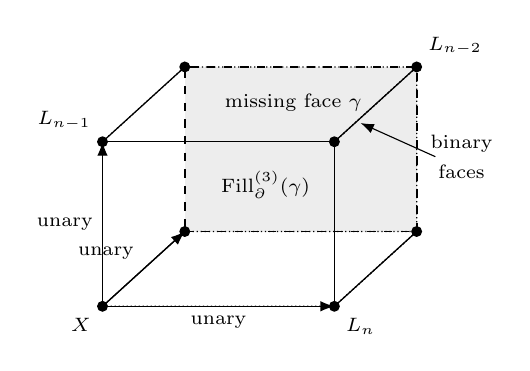
\begin{tikzpicture}[scale=0.95,>=Latex,
  vertex/.style={circle,fill=black,inner sep=1.4pt},
  edge/.style={line width=0.45pt},
  unary/.style={edge,->},
  face/.style={edge,densely dotted},
  missing/.style={edge,dashed,line width=0.7pt}]

\coordinate (x0) at (0,0);
\coordinate (x1) at (3.1,0);
\coordinate (x2) at (0,2.2);
\coordinate (x3) at (3.1,2.2);
\coordinate (y0) at (1.1,1.0);
\coordinate (y1) at (4.2,1.0);
\coordinate (y2) at (1.1,3.2);
\coordinate (y3) at (4.2,3.2);

\fill[gray!14] (y0)--(y1)--(y3)--(y2)--cycle;
\draw[edge] (x0)--(x1)--(x3)--(x2)--cycle;
\draw[edge] (x0)--(y0) (x1)--(y1) (x2)--(y2) (x3)--(y3);
\draw[missing] (y0)--(y1)--(y3)--(y2)--cycle;

\draw[unary] (x0)--node[below] {\scriptsize unary} (x1);
\draw[unary] (x0)--node[left] {\scriptsize unary} (x2);
\draw[unary] (x0)--node[above left] {\scriptsize unary} (y0);

\draw[face] (x1)--(y1)--(y3)--(x3);
\draw[face] (x2)--(y2)--(y3)--(x3);
\draw[face] (x0)--(x1)--(y1)--(y0);

\foreach \p in {x0,x1,x2,x3,y0,y1,y2,y3} \node[vertex] at (\p) {};

\node[below left=1pt of x0] {\scriptsize \(X\)};
\node[below right=1pt of x1] {\scriptsize \(L_n\)};
\node[above left=1pt of x2] {\scriptsize \(L_{n-1}\)};
\node[above right=1pt of y3] {\scriptsize \(L_{n-2}\)};

\node at (2.55,2.72) {\scriptsize missing face \(\gamma\)};
\node at (2.18,1.62) {\scriptsize \(\mathrm{Fill}^{(3)}_{\partial}(\gamma)\)};
\node[align=center] at (4.8,2.0) {\scriptsize binary\\[-1pt]\scriptsize faces};
\draw[->] (4.45,2.0)--(3.45,2.45);
\end{tikzpicture}
\caption{A depth-three structural open box.  Unary action data and already exported binary
comparison faces determine the boundary \(\partial\); the shaded back face is the missing
remote comparison \(\gamma\), and the interior cell is the filler computed by the cubical
operations.}
\label{fig:depth-three-open-box}
\end{figure}

\subsection{Derivedness and minimal public signatures}
\label{subsec:derivedness-minimal-signatures}

The open-box theorem is semantic.  It says that the higher exact factor is contractible.  The
public-signature theorem is syntactic-accounting.  It says that an explicit higher structural
field in a surface presentation can be replaced by the cubically computed term and therefore
removed from the primitive part of a \(\mu\)-minimal signature.

The bridge between the two levels is the computational replacement theorem from
Section~3: when a presented field is accompanied by a uniform derivation from lower public
boundary data, the presentation relation allows the field to be replaced by that derived term.
The open-box theorem supplies exactly such a derivation for higher structural trace.

\begin{thm}[Derived trace witnesses for higher structural horns]
\label{thm:higher-structural-derived-trace}
Let \(h\) be a normalized structural horn package generated by the fixed cubical
sealed-extension grammar, and suppose the historical arity of \(h\) is at least three.  Then
\(h\) carries a derived trace witness in the sense of
Definition~\ref{def:derived-trace-witness}.

Dependencies: syntactic horn reduction, horn-to-open-box adequacy, total open-extension
contractibility, substitution stability, and computational replacement on canonical trace
presentations.

Proof contract: the input is a normalized higher structural horn package; the
constructed output is the full \(\mathsf{DerivedTrace}\) witness for that
package.  The proof uses the horn-reduction and horn-to-open-box induction
results to expose the extension object, then uses the open-box contraction to
choose the replacement term.  Cubical operations enter through the computed
center and its transport back across the horn/open-box equivalence.  The
allowed dependencies are exactly the lower public boundary of the horn.
Artifact status: conditional on adequacy.  Without this theorem, higher fields
could only be called derived by convention, not by a checkable witness.
\end{thm}

\begin{proof}
Let \(\partial_h\) be the lower public boundary of \(h\).  By
Lemma~\ref{lem:syntactic-horn-reduction}, the exact additional datum represented by \(h\) is
a dependent sum
\[
  \sum_{\gamma:\Gamma_{\mathrm{miss}}(\partial_h)}
    \mathsf{Fill}_{\partial_h}(\gamma).
\]
By Lemma~\ref{lem:horn-open-box}, this sum is equivalent to the explicit structural
open-box extension decoded from the horn grammar.  The decoded box exposes the family
\(A\), the face formula \(\varphi\), the partial boundary \(u\), the base face \(u_0\), the
compatible lid subtype, and the filler family.

Theorem~\ref{thm:open-ext-contr} gives a canonical center of this open-box extension,
computed by cubical composition and filling.  Transporting that center back along the
horn-to-open-box equivalence gives the replacement term
\[
  t_h(\partial_h)
  :
  \sum_{\gamma:\Gamma_{\mathrm{miss}}(\partial_h)}
    \mathsf{Fill}_{\partial_h}(\gamma).
\]
The typing and boundary equations are the endpoint and side equations of the decoded
open box.  Semantic preservation is the equivalence of
Lemma~\ref{lem:horn-open-box}.  The allowed-dependency condition holds because the decoded
box is assembled from \(\partial_h\) and the fixed cubical operations only.  Substitution
stability is Lemma~\ref{lem:open-box-substitution}.  Finally, public-normalization
compatibility is exactly the hypothesis consumed by the computational replacement theorem of
Section~3: replacing the explicit horn field by the computed center gives a presentation of
the same canonical trace signature in which the horn field is derived rather than primitive.
These are precisely the components required by
Definition~\ref{def:derived-trace-witness}.
\end{proof}

\begin{thm}[Minimal-signature elimination above binary arity]
\label{thm:minimal-signature-elimination}
Let \(e\) be an admissible surface extension declaration over \(B_n\).  Then there exists a
presentation-equivalent declaration \(e'\approx e\) whose normalized trace signature contains
no irreducible primitive historical field of arity \(k\geq 3\).  Equivalently, every canonical
\(\mu\)-minimal normalized public signature contains only unary and binary primitive
structural trace fields.

More concretely, if a presented structural field of arity \(k\geq 3\) occurs in some surface
declaration, then in the canonical trace-presentation interface it is transparently derived
from its lower-arity boundary by a term synthesized from cubical composition, transport, and
filling.

Dependencies: normal-form classification, derived trace witnesses for higher structural
horns, and the computational replacement theorem.

Proof contract: the input is an admissible surface declaration and any
apparent primitive structural field of arity at least three; the constructed
output is a presentation-equivalent declaration with that field replaced by its
derived term, iterated over all such fields.  The induction is finite induction
over the normalized trace telescope, using the horn-derivedness theorem at each
step.  Cubical operations enter only through the supplied replacement witnesses,
and those witnesses are lower-boundary dependent.  Artifact status: conditional
on adequacy.  Without this theorem, exact contractibility would not imply the
\(\mu\)-minimal public-signature bound.
\end{thm}

\begin{proof}
Fix a presentation of \(e\) and an apparent primitive structural trace field \(\phi\) of arity
\(k\geq 3\) in its elaborated sealed export.  By the normal-form classification of Section~4,
\(\phi\) is a higher structural horn package rather than payload.  By
Theorem~\ref{thm:higher-structural-derived-trace}, \(\phi\) carries a
\(\mathsf{DerivedTrace}\) witness.  Concretely, this witness supplies lower boundary data
\(\partial\), the replacement term \(t_\phi(\partial)\), typing and boundary equations,
semantic preservation, allowed-dependency data, substitution stability, and
public-normalization compatibility.

The computational replacement rule of Section~3 then applies: a presented higher structural
field equipped with such a uniform lower-boundary derivation is presentation-equivalent to
the declaration in which the field is replaced by \(t_{\phi}(\partial)\) and classified as
derived by the supplied witness.
Repeating this replacement for every arity-\(k\geq 3\) structural field terminates because the
normalized signature is finite.  The resulting presentation-equivalent declaration \(e'\) has
no primitive structural field above binary arity.  Since \(\mu\) counts only primitive trace
fields in canonical normal form, every \(\mu\)-minimal signature has the same property.
\end{proof}

\begin{defi}[Primitive status and minimal opaque cost]
\label{def:primitive-status-mu}
After the replacement procedure of Theorem~\ref{thm:minimal-signature-elimination}, an atomic
trace schema in a normalized public signature is \emph{derived} if it is synthesized by
transparent normalization, by generic cubical structure, or by a supplied
\(\mathsf{DerivedTrace}\) witness.  It is \emph{primitive} if no such synthesis is available in
the fixed normalization relation.  For an admissible declaration \(e\), let
\(N_{\mathrm{tr}}^{\mathrm{prim}}(e)\) be the resulting primitive trace part.  The minimal
opaque public trace cost is
\[
  \mu(e)
  :=
  \min\{\, |N_{\mathrm{tr}}^{\mathrm{prim}}(e')| \mid e'\approx e \,\}.
\]
This is the formal version of the accounting notation introduced in
Definition~\ref{def:mu-provisional}; in particular, \(\mu\) is attached to canonical
normalized public signatures after witnessed replacement, not to raw declarations.
\end{defi}

\begin{rem}[What is eliminated]
Theorem~\ref{thm:minimal-signature-elimination} eliminates primitive public fields, not exact
semantic factors.  A higher horn factor may still occur in \(\mathrm{Real}_k(X)\), but after
Theorem~\ref{thm:open-ext-contr} it occurs as a contractible factor with a canonical center.
The trace-cost invariant \(\mu\) does not count such a factor as primitive public trace.
\end{rem}

\subsection{Exact stabilization above binary trace}
\label{subsec:exact-stabilization}

We can now prove the upper bound on obligation depth.  The proof is conceptually simple:
from depth two onward, each further exposure of remote history adjoins one structural
open-box extension factor; each such factor is contractible; dependent sums with
contractible fibers are equivalent to their bases.

\begin{lem}[Kan contraction for horn fibers]
\label{lem:kan-contraction-horn-fibers}
For every structural horn-extension fiber \(H_k(\partial)\) generated by the fixed cubical
sealing grammar, the projection
\[
  H_k(\partial) \to 1
\]
is contractible in the cubical metatheory.  The center is the missing face and filler computed
from \(\partial\) by the cubical operations.

Dependencies: horn-to-open-box adequacy and total open-extension contractibility.

Proof contract: the input is a generated horn fiber \(H_k(\partial)\); the
constructed output is its canonical center and contraction.  No new induction
is used: the proof composes the horn-to-open-box equivalence with total
open-extension contractibility.  Cubical operations enter through the
open-extension center, and the only data consumed from \(\partial\) are the
lower public boundary faces.  Artifact status: mechanized for an abstract
interface.  Without this lemma, each step from \(\Real_k\) to
\(\Real_{k-1}\) would lack a contractible fiber.
\end{lem}

\begin{proof}
By Lemma~\ref{lem:horn-open-box}, \(H_k(\partial)\) is the open-box extension type for the
structural tuple
\[
  (A_k,\varphi_k,u_k,u^0_k).
\]
Applying
Theorem~\ref{thm:open-ext-contr} gives a canonical center and a contraction of the whole
extension space.  Presentation equivalence is not used to prove this contractibility; it is
used only in Theorem~\ref{thm:minimal-signature-elimination} to classify the corresponding
public field as derived.
\end{proof}

\begin{thm}[Exact stabilization of realized structural obligations]
\label{thm:exact-stabilization}
In the fixed cubical extension calculus, for every foundational-core candidate \(X\) and
every \(k\geq 2\) the restriction map
\[
  \res_{2,k}(X):\mathrm{Real}_k(X)\longrightarrow\mathrm{Real}_2(X)
\]
is an equivalence.  Its inverse
\[
  \ext_{2,k}(X):\mathrm{Real}_2(X)\longrightarrow\mathrm{Real}_k(X)
\]
is constructed by structural recursion over the generated obligations of arity
greater than two, adjoining for each such obligation the canonical center of
the decoded total open-extension object.  The composites
\(\res_{2,k}\circ\ext_{2,k}\) and \(\ext_{2,k}\circ\res_{2,k}\) are identified
with the corresponding identities by the contraction paths of those
open-extension fibers.
Consequently \(d_{\mathrm{obl}}\leq 2\).

Dependencies: the formal definition of \(\mathrm{Real}_k\), arity-cell identification,
syntactic horn reduction, horn-to-open-box adequacy, and total open-extension
contractibility.

Proof contract: the input is a depth-two realization and a bound \(k\geq 2\);
the constructed output is \(\ext_{2,k}\), together with the two equivalence
laws for \(\res_{2,k}\).  The proof is induction on the depth index, using the
structural horn fiber exposed at each successor step.  Cubical operations enter
only through the canonical centers and contraction paths of those fibers.  Each
successor step uses the lower-depth realization as its boundary and does not
inspect private derivations.  Artifact status: mechanized for an abstract
interface.  Without this theorem, the upper bound \(d_{\mathrm{obl}}\leq 2\)
would not follow.
\end{thm}

\begin{proof}
The case \(k=2\) is immediate.  For \(k=3\), Lemmas~\ref{lem:arity-cell} and
\ref{lem:syntactic-horn-reduction} identify the marginal depth-three datum over each
boundary \(\partial:\mathrm{Real}_2(X)\) as the horn-extension fiber \(H_3(\partial)\).  Hence
\[
  \mathrm{Real}_3(X)
  \simeq
  \sum_{\partial:\mathrm{Real}_2(X)} H_3(\partial).
\]
By Lemma~\ref{lem:kan-contraction-horn-fibers}, every fiber \(H_3(\partial)\) is
contractible.  A dependent sum over a family of contractible fibers is canonically equivalent
to its base, so
\[
  \mathrm{Real}_3(X) \simeq \mathrm{Real}_2(X).
\]

For \(k>3\), the same argument repeats.  Passing from depth \(k-1\) to depth \(k\) exposes
one additional remote layer and adjoins one structural horn-extension fiber \(H_k(\partial)\)
over \(\partial:\mathrm{Real}_{k-1}(X)\).  Lemma~\ref{lem:kan-contraction-horn-fibers}
contracts that fiber, so
\[
  \mathrm{Real}_k(X) \simeq \mathrm{Real}_{k-1}(X)
  \qquad (k\geq 3).
\]
Iterating these equivalences yields \(\mathrm{Real}_k(X)\simeq\mathrm{Real}_2(X)\) for all
\(k\geq 2\).  Written as maps, the forward map is the telescope projection
\(\res_{2,k}(X)\).  The inverse \(\ext_{2,k}(X)\) starts with
\(\partial:\mathrm{Real}_2(X)\) and repeatedly adjoins the canonical center of each
successive horn-extension fiber \(H_j(\partial_j)\), for \(3\leq j\leq k\).
The first round trip is judgmentally the identity on the retained depth-two
fields.  The second round trip is homotopic to the identity because each
discarded higher component is connected to the canonical center by the
contraction supplied by Lemma~\ref{lem:kan-contraction-horn-fibers}.
\end{proof}

\begin{cor}[Contractible-factor decomposition]
\label{cor:contractible-factor-decomposition}
For every foundational-core candidate \(X\) and every \(k\geq 2\), there is a canonical
equivalence
\[
  \mathrm{Real}_k(X)
  \simeq
  \mathrm{Real}_2(X) \times C_k(X),
\]
where \(C_2(X):=1\) and, for \(k>2\), \(C_k(X)\) is the iterated chain of canonical remote
horn factors selected by the cubical compositions in the proof of
Theorem~\ref{thm:exact-stabilization}.  Each \(C_k(X)\) is canonically contractible.

Dependencies: exact stabilization and Kan contraction for structural horn fibers.

Proof contract: the input is the exact-stabilization equivalence; the
constructed output is an explicit contractible-factor decomposition of the
higher part.  The proof reuses the depth-index induction of
Theorem~\ref{thm:exact-stabilization}.  Cubical operations enter through the
chosen centers of the horn fibers, and every factor is lower-boundary
dependent.  Artifact status: mechanized for an abstract interface.  Without
this corollary, the reader would see stabilization but not the residual
contractible higher factors.
\end{cor}

\begin{proof}
The proof of Theorem~\ref{thm:exact-stabilization} trivializes each successive horn-extension
fiber by choosing its canonical cubical center.  Iterating those choices identifies the total
higher part with a product of the depth-two boundary and the chain of chosen remote horn
factors.  Each factor is contractible by Lemma~\ref{lem:kan-contraction-horn-fibers}, hence
the whole chain \(C_k(X)\) is contractible.
\end{proof}

The corollary expresses the exact semantic situation more vividly than the bare equivalence:
above depth two there may be additional exact factors, but all of them are canonical and
contractible.  The primitive public signature sees only the depth-two part.

\subsection{The lower bound: univalence forces binary trace}
\label{subsec:swap-lower-bound}

It remains to show that the upper bound is exact.  The obstruction is small but decisive.
A univalent interface that exports the two-point type also exports the path corresponding to
its nontrivial automorphism.  A sealed action must respect that path.  Objectwise unary data
alone cannot express this naturality condition.  This is the lower-bound branch of the
running example from the introduction.

\begin{defi}[Unary and binary fragments for the swap test]
\label{def:swap-unary-binary-fragments}
For a candidate \(X\) over the two-point interface, the unary fragment
\(\Real_1(X)\) records only the objectwise action field
\[
  F_2:2\to 2.
\]
The binary fragment \(\Real_2(X)\) extends this record by the comparison field forced by the
exported univalent swap path:
\[
  \alpha_{\mathrm{swap}}:
  \mathrm{transport}_{\lambda A. A\to A}(p_{\mathrm{swap}},F_2)=F_2.
\]
The map \(\res_{1,2}:\Real_2(X)\to\Real_1(X)\) forgets
\(\alpha_{\mathrm{swap}}\).  Thus a unary-accepted candidate is an inhabitant of
\(\Real_1(X)\), while binary acceptance asks for a point in the fiber of
\(\res_{1,2}\) over that unary action.
\end{defi}

\begin{thm}[Explicit binary sealing obstruction]
\label{thm:swap-obstruction}
Let the active interface of a univalent foundation export the two-point type \(2\) and the
univalent path
\[
  p_{\mathrm{swap}} := \mathrm{ua}(\mathrm{swap}) : 2 = 2.
\]
Then there is a candidate \(X_{\mathrm{const}}\) and an element
\[
  x_1:\Real_1(X_{\mathrm{const}})
\]
such that the fiber
\[
  \sum_{x_2:\Real_2(X_{\mathrm{const}})}
  \res_{1,2}(x_2)=x_1
\]
is empty.  Equivalently, the unary fragment admits a raw objectwise action that the binary
fragment rejects.  Consequently depth-one data are insufficient in general, and
\(d_{\mathrm{obl}}\geq 2\).

Dependencies: the univalent two-point interface, transport in the endomorphism family, and
the distinction between unary objectwise action and binary sealing naturality.

Proof contract: the input is the public two-point type with its univalent swap
path; the constructed output is a unary point whose binary fiber is empty.  No
structural induction is used.  Cubical structure enters through univalence and
transport in \(A\mapsto A\to A\), which computes conjugation by swap.  The
argument uses only unary objectwise data and the single public binary path, so
there is no hidden higher dependency.  Artifact status: fully mechanized.
Without this theorem, the upper bound could collapse to a merely unary result.
\end{thm}

\begin{proof}
Consider an active-interface package consisting of an endomap on the exported two-point
type:
\[
  X_{\mathrm{act}} := (F_2 : 2\to 2).
\]
The unary candidate chooses the constant-left map
\[
  F_2 := \lambda\_.\,\mathsf{left}.
\]
This is a well-formed objectwise clause, so it determines the point
\(x_1:\Real_1(X_{\mathrm{const}})\).  But sealing a globally acting structural extension
requires compatibility with exported paths.  Since the old public interface exports
\(p_{\mathrm{swap}}\), the binary naturality obligation in \(\Real_2(X_{\mathrm{const}})\) is
\[
  \alpha_{\mathrm{swap}}:
  \mathrm{transport}_{\lambda A. A\to A}(p_{\mathrm{swap}},F_2)=F_2.
\]
By univalence, transport in the endomorphism family along \(p_{\mathrm{swap}}\) computes by
conjugation with the swap equivalence.  Therefore
\[
  \mathrm{transport}_{\lambda A. A\to A}(p_{\mathrm{swap}},F_2)
  =
  \mathrm{swap}\circ F_2\circ \mathrm{swap}^{-1}
  =
  \lambda\_.\,\mathsf{right}.
\]
Thus \(\alpha_{\mathrm{swap}}\) would be an equality
\[
  (\lambda\_.\,\mathsf{right})=(\lambda\_.\,\mathsf{left}),
\]
which is impossible because evaluating at \(\mathsf{left}\) would force
\(\mathsf{right}=\mathsf{left}\).

There is also a positive control: if \(F_2\) is the identity map, conjugation along swap
returns the identity map, and the binary obligation is inhabited.  The failure of the
constant-left map is therefore not a defect of the formulation; it is the type checker
detecting an objectwise action that does not respect exported path structure.  Hence the
fiber of \(\res_{1,2}\) over the constant-left unary point is empty: \(\Real_1\) can be
inhabited while the corresponding \(\Real_2\) extension is impossible.  Thus
\(\Real_1\) and \(\Real_2\) are not canonically equivalent in general, and the obligation
depth cannot be one.
\end{proof}

\begin{rem}[Adjunctions as an explanatory analogue]
Adjunctions exhibit the same binary pattern categorically.  Once the object action and the
unit/counit data have been fixed, the triangle identities compare composites already
determined at the unary level.  The paper uses this only as an analogy.  The internal lower
bound for the fixed cubical calculus is the swap obstruction of
Theorem~\ref{thm:swap-obstruction}.
\end{rem}

\subsection{Exact public structural depth two}
\label{subsec:exact-depth-two-conclusion}

We can now combine the upper and lower bounds.

\begin{cor}[Fixed-calculus exact structural integration depth two]
\label{cor:exact-depth-two}
In the fixed cubical sealed-extension calculus, admissible sealed structural extensions have
exact structural integration depth two:
\[
  d_{\mathrm{obl}}=2.
\]
Moreover every \(\mu\)-minimal normalized public signature contains no primitive structural
trace field of historical arity greater than two.

Dependencies: exact stabilization for the upper bound, minimal-signature elimination for
the public-signature statement, and the swap obstruction for the lower bound.

Proof contract: the input is an admissible sealed structural extension of the
fixed calculus; the constructed output is the exact equality
\(d_{\mathrm{obl}}=2\) plus the \(\mu\)-minimal public-signature bound.  The
proof uses no new induction: it combines the depth-index induction of
Theorem~\ref{thm:exact-stabilization}, the replacement theorem, and the swap
lower bound.  Cubical operations enter through those cited results, and all
higher dependencies have already been reduced to lower public boundaries.
Artifact status: conditional on adequacy.  Without this corollary, the paper
would contain separate upper, lower, and accounting claims but no single exact
depth statement.
\end{cor}

\begin{proof}
Theorem~\ref{thm:exact-stabilization} gives the upper bound
\(d_{\mathrm{obl}}\leq 2\) by showing
\(\mathrm{Real}_k(X)\simeq\mathrm{Real}_2(X)\) for all \(k\geq 2\).  Theorem~\ref{thm:minimal-signature-elimination}
turns the same cubical horn computation into the public-signature statement
\(d_\mu\leq 2\).  Finally, Theorem~\ref{thm:swap-obstruction} gives the lower bound
\(d_{\mathrm{obl}}\geq 2\) by exhibiting a genuine binary sealing obstruction in the univalent
setting.  Hence the exact obligation depth is two.
\end{proof}

The result should be read with the distinctions of Remark~\ref{rem:five-statuses} in mind.
Higher structural exact factors do not vanish from the semantics; they stabilize as
contractible open-box extension factors.  What disappears from the primitive public
interface is the need to present those factors as irreducible fields.  This is the semantic
content behind the paper's summary:
\[
  \text{binary trace is necessary; higher structural trace is computed.}
\]

\section{Mechanization and trusted boundary}
\label{sec:mechanization}

The artifact checks the theorem-facing fixed-calculus stack and records the
boundary between checked Agda statements, abstract interfaces, and paper-level
adequacy assumptions.  The detailed artifact guide and auxiliary walkthroughs
are intentionally kept out of the LMCS paper and belong to the archived release.

The paper and the machine-readable theorem map use the following four status
phrases.  A claim is \emph{fully mechanized} when the named Agda modules check
the claim directly for the fixed object under discussion, with no local
postulates or local primitive declarations beyond the trusted cubical library.
It is \emph{mechanized for an abstract interface} when Agda checks a precise
interface theorem, but an instantiation or adequacy argument is a separate
input.  It is \emph{conditional on adequacy} when checked components are present
but the paper-level claim depends on the stated bridge from surface
presentations or semantic wrappers to \(C_{\mathrm{ext}}\).  It is
\emph{paper-only} when the item is an expository, release, or future-transfer
claim rather than a theorem checked by the artifact.

For this submission, \texttt{paper-map.yaml} remains the machine-readable theorem map for the
full repository paper source.  The LMCS file deliberately compresses several labels into the
table below; the bridge from those compressed LMCS references back to the checked Agda surface
is documented in the repository theorem index rather than by retargeting the existing checker.

\begin{center}
\scriptsize
\setlength{\tabcolsep}{2pt}
\begin{tabular}{p{0.17\linewidth}p{0.15\linewidth}p{0.18\linewidth}p{0.27\linewidth}p{0.16\linewidth}}
\hline
Paper claim & LMCS reference & Status & Artifact surface & Trusted input or condition \\
\hline
Fixed calculus and generated obligations
& Section~\ref{sec:fixed-calculus}, Definition~\ref{def:generated-structural-obligations}
& fully mechanized
& raw structural syntax/typing and normalization bridge modules
& fixed raw syntax and Cubical library \\
\hline
\(\mathrm{ObSig}_k\), \(\mathrm{Real}_k\), restriction, and stabilization
& Definition~\ref{def:obsig-real}, Theorem~\ref{thm:exact-stabilization}
& mechanized for an abstract interface
& upper-bound and semantic exact-depth modules
& theorem-facing realization and horn interfaces \\
\hline
Horn-to-open-box decoding
& Lemma~\ref{lem:horn-open-box}
& mechanized for an abstract interface
& structural horn decoding and open-box bridge modules
& generated horn grammar; raw/surface use needs the bridge \\
\hline
Total open-extension contractibility
& Theorem~\ref{thm:open-ext-contr}
& mechanized for an abstract interface
& cubical open-box extension, contraction, and substitution modules
& cubical \(\mathsf{hcomp}\), \(\mathsf{hfill}\), and \(\mathrm{Partial}/\mathrm{Sub}\);
not fixed-lid uniqueness \\
\hline
Derived-trace replacement and \(\mu\)-minimal elimination
& Theorems~\ref{thm:higher-structural-derived-trace}
and~\ref{thm:minimal-signature-elimination}
& conditional on adequacy
& normalization-derived, replacement, and computational-replacement modules
& canonical trace presentations and fixed raw bridge \\
\hline
Binary lower bound
& Theorem~\ref{thm:swap-obstruction}
& fully mechanized
& adjunction-barrier, depth-lower-bound, and exact-depth modules
& univalence and the two-point swap interface \\
\hline
Exact public depth-two conclusion
& Corollary~\ref{cor:exact-depth-two}
& conditional on adequacy
& exact-depth wrappers plus replacement modules
& adequacy bridge for public signatures \\
\hline
Broad transfer to arbitrary cubical languages
& non-claim
& paper-only
& no theorem in this artifact
& external parser/elaborator and semantic adequacy theorem required \\
\hline
\end{tabular}
\end{center}

The trusted base consists of the Agda kernel with cubical support, the pinned
Cubical Agda library used by the repository, the fixed raw extension-calculus
records that define \(C_{\mathrm{ext}}\), and the small support libraries used by
the checked theorem-facing modules.  The theorem map audits the theorem-facing import
closure for local postulates and local primitive declarations; imported cubical
primitives remain part of the trusted library base.  A checked module therefore
supports exactly the row in which it appears.  It does not by itself claim that
every surface language or every cubical foundation instantiates the fixed
interface.

The archived artifact contains the paper source, Agda modules, theorem map, and
audit scripts.  Reviewers can run the aggregate check
from the release root; it typechecks the theorem-facing aggregate, verifies the
paper-to-Agda map, and audits the theorem-facing import closure for local
postulates and primitive declarations.  The development repository is not the
archival citation.  The archived artifact for this submission is identified by
the Zenodo DOI
\href{https://doi.org/10.5281/zenodo.20235005}{10.5281/zenodo.20235005}.
The final archival tag and hosted artifact-check URL are release metadata, not
additional theorem claims.


\section{Conclusion}

This paper proves an exact depth-two theorem for the fixed cubical
sealed-extension calculus \(C_{\mathrm{ext}}\).  Unary trace is insufficient:
univalence exposes public comparisons, and the two-point swap gives a concrete
binary sealing obstruction.  Trace above binary arity is still present in the
exact semantic object, but it is represented as a cubical open-box extension
factor and is contractible over its lower boundary.  Computational replacement
therefore removes such fields from \(\mu\)-minimal normalized public signatures.

The binary boundary is exact because it is where public comparison first enters.
Objectwise action is unary, but naturality along a public equivalence is binary.
In the running two-point example, the constant-left action exposes the lower
bound by failing this comparison, while the identity action shows the positive
branch on which higher questions can be asked.  After that binary boundary is
present, sealing-generated higher coherence data has the shape cubical
composition is designed to fill: lower faces are public, the missing face is
computed, and the filler is canonical up to the contractibility proved in the
fixed interface.

The scope is the one fixed in Section~\ref{subsec:scope-nongoals}: transfer to
other foundations requires the stated adequacy and normalization interface.  The
mechanization records this trusted boundary rather than hiding it.

Future work is to instantiate the interface for broader cubical foundations
and turn the current adequacy bridges into reusable criteria for structural
extensions.



\bibliographystyle{alphaurl}
\bibliography{coherence_depth_refs}

\end{document}
